\documentclass[12pt]{article}
\usepackage[utf8]{inputenc}
\usepackage[T1]{fontenc}
\usepackage{geometry}
\usepackage{graphicx}
\usepackage{makeidx}
\usepackage{amsmath}
\geometry{margin=2.5cm}

\title{Informe - Práctica \#2}
\author{Tu nombre}
\date{Fecha de entrega}

\begin{document}
	
	\thispagestyle{empty}
	
	\begin{center}
		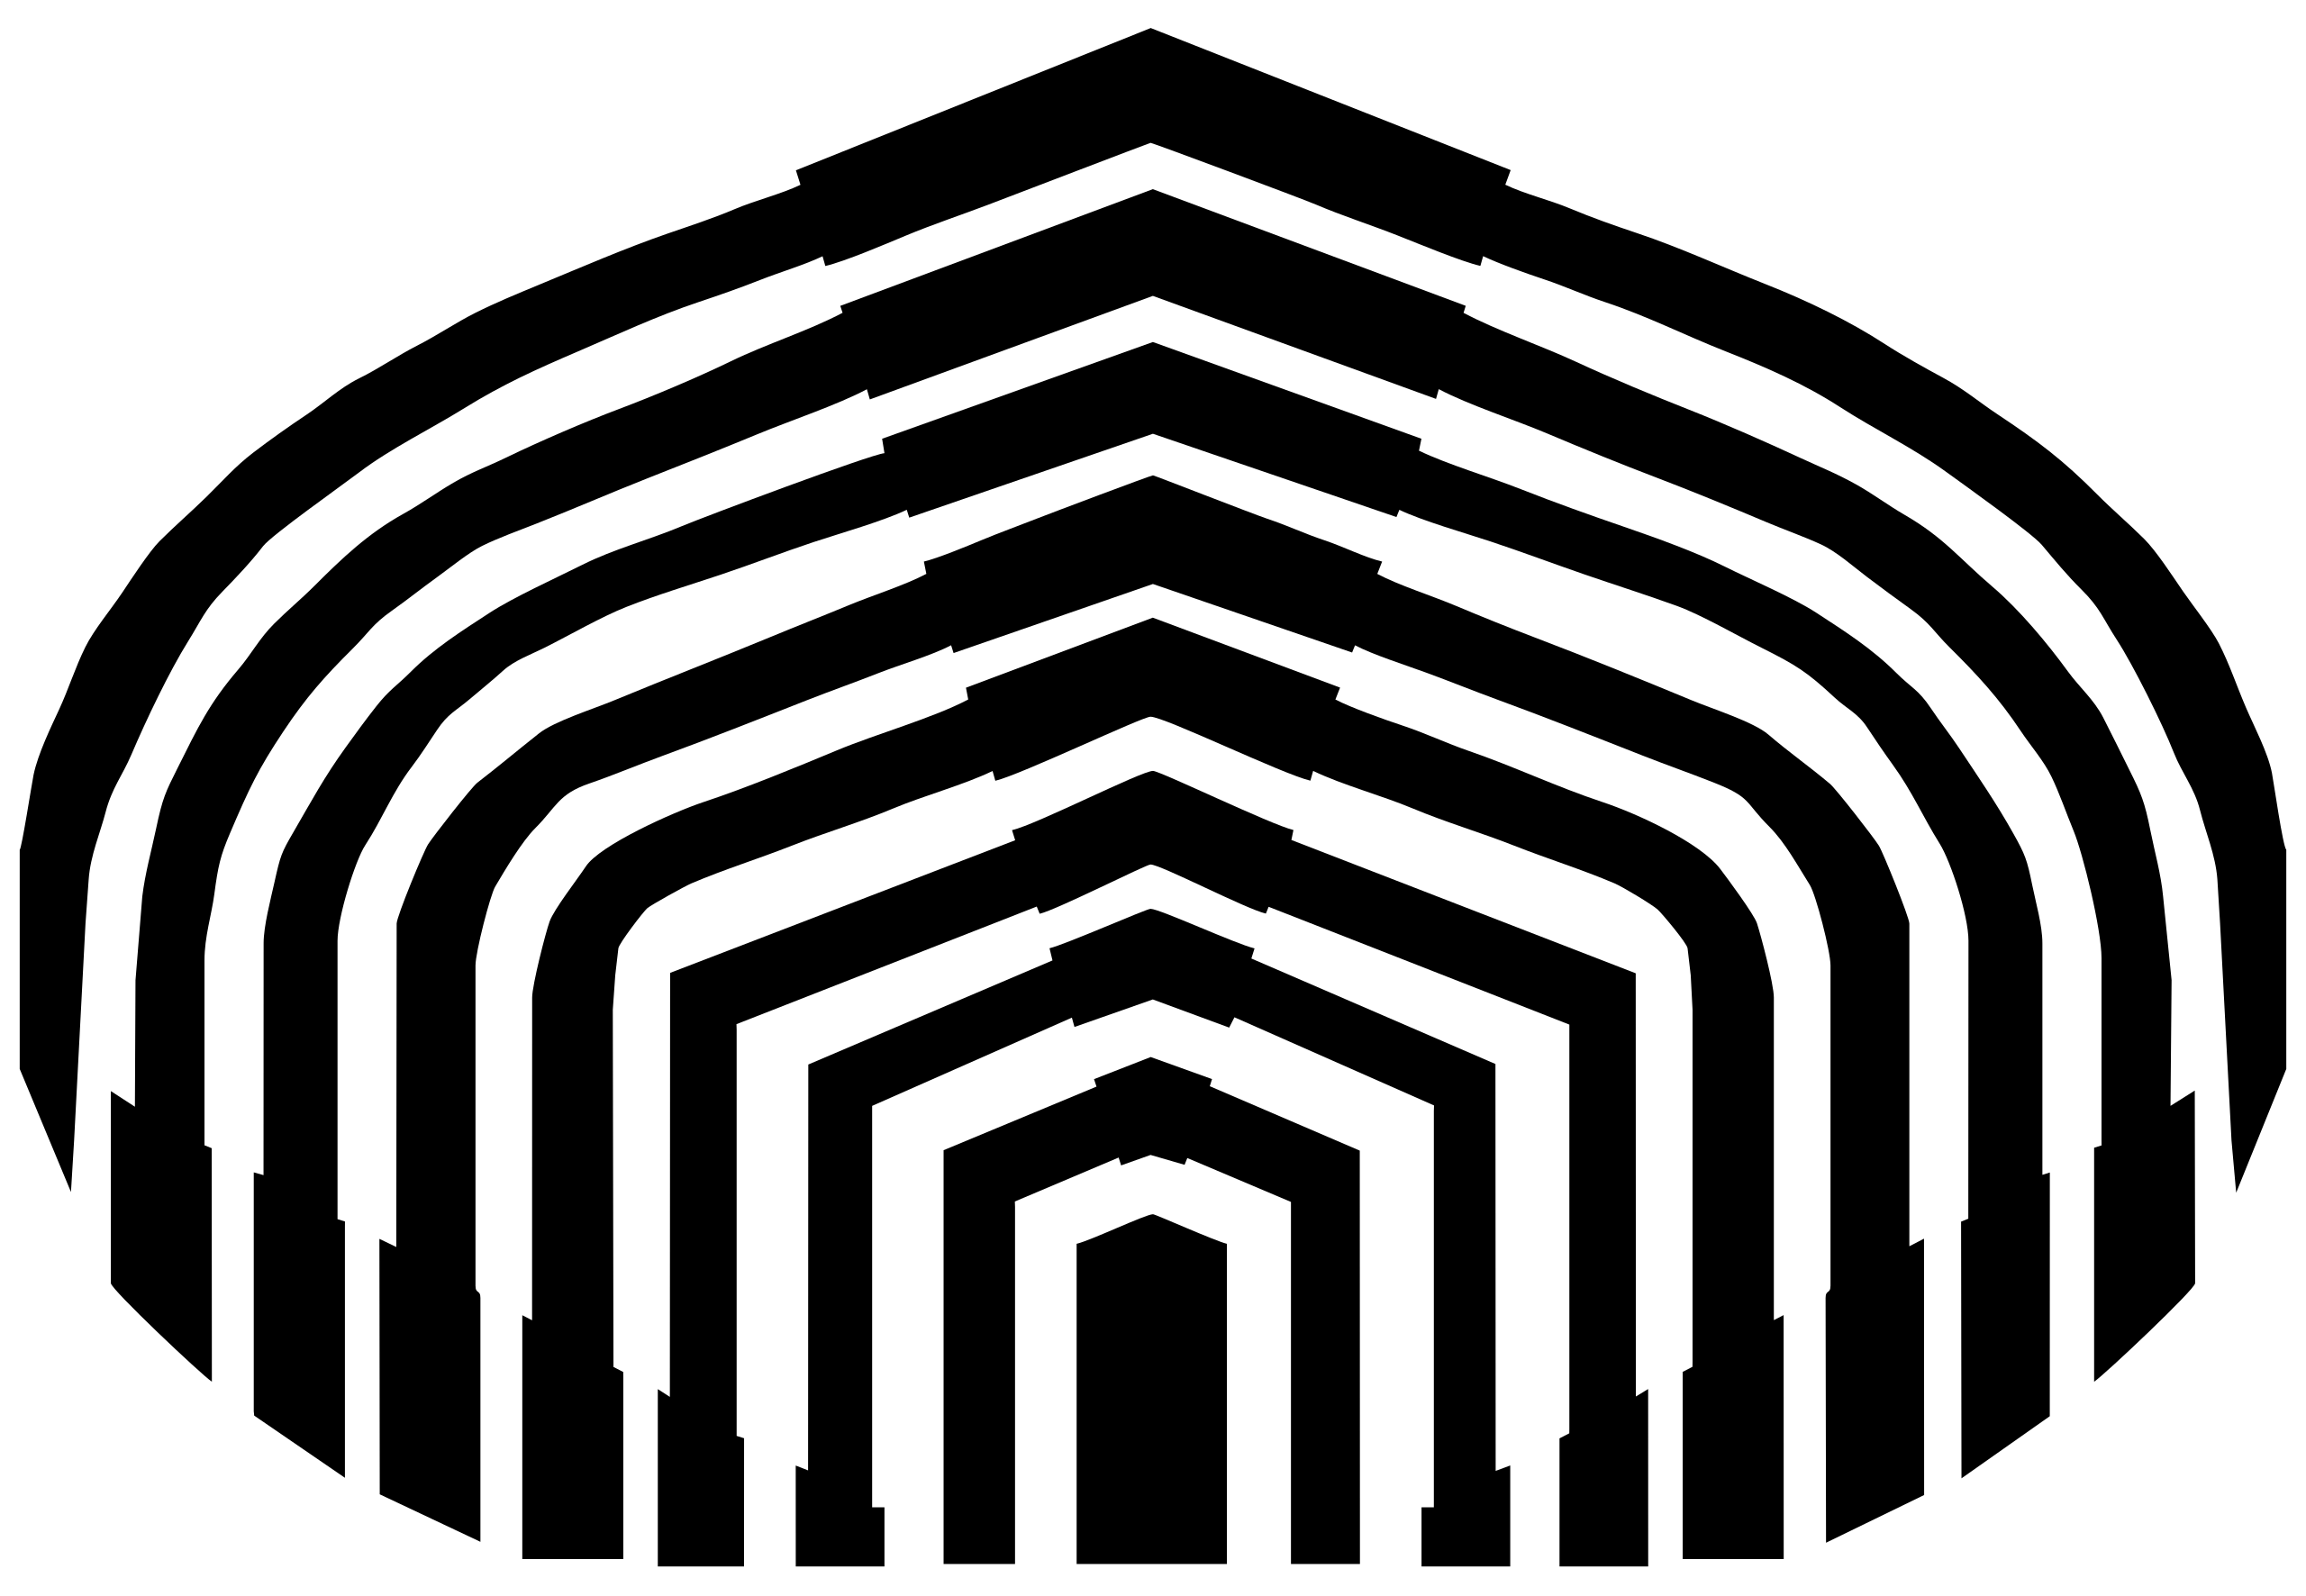
\includegraphics[width=3.1cm,height=2cm]{logo}\\
		UNIVERSIDAD SIMÓN BOLÍVAR\\
		DEPARTAMENTO DE ELECTRÓNICA Y CIRCUITOS\\
		EC1281 - LABORATORIO DE MEDICIONES ELÉCTRICAS\\
		SECCIÓN 1 - GRUPO 1\\
		
		\vspace{7cm}
		\textbf{\Large INFORME - PRÁCTICA \#2}\\
		SIMULACIÓN DE CIRCUITOS CON SPICE\\
	\end{center}
	
	\begin{flushleft}
		\vspace{9cm}
		\hfill Integrantes:\\
		\hfill {\large Luis Becerra - 1910557}\\
		\hfill {\large Lorena Rojas - 1910469}\\
	\end{flushleft}
	
	\newpage
	
	\pagenumbering{roman}
	
	\begin{center}
		\textbf{\large RESUMEN}\\
	\end{center}
	
	En el laboratorio de esta semana, nos familiarizamos con el programa PSPICE y exploramos una variedad de circuitos utilizando diferentes componentes y fuentes de voltaje. Comenzamos nuestro estudio con fuentes de corriente y resistencias en serie, lo que nos permitió comprender las características básicas de los circuitos eléctricos. A medida que avanzamos, pasamos a trabajar con fuentes de corriente alterna y utilizamos condensadores e inductores para analizar su comportamiento en el dominio de la frecuencia. Además, experimentamos reemplazando las fuentes de corriente alterna por fuentes de pulso en estos circuitos para obtener diferentes resultados.\\
	
	Exploramos también circuitos trifásicos en configuraciones estrella-estrella y estrella-delta, lo que nos permitió comprender el flujo de corriente en sistemas de energía trifásica. Por último, abordamos el diseño de circuitos con amplificadores operacionales (OPAM), específicamente filtros pasa-bajo y pasa-alto activos. Utilizamos los análisis disponibles en PSPICE, como el análisis transitorio, el análisis de punto de polarización y el análisis de barrido de frecuencia, para obtener una comprensión completa del comportamiento de los circuitos en diferentes condiciones.\\
	
	En resumen, este laboratorio nos brindó una sólida introducción al uso de PSPICE y nos permitió explorar una variedad de circuitos con diferentes componentes y fuentes de voltaje. A través de nuestros experimentos y análisis, adquirimos un mayor conocimiento sobre el comportamiento de los circuitos eléctricos y sus aplicaciones prácticas.\\
	
	\newpage
	
	\begin{center}
		\textbf{\large ÍNDICE}\\
	\end{center}
	
	\noindent \textbf{RESUMEN} \hfill \textbf{I}\\
	\noindent \textbf{ÍNDICE} \hfill \textbf{II}\\
	\noindent \textbf{MARCO TEÓRICO} \hfill \textbf{1}\\
	\noindent \textbf{METEODOLOGÍA} \hfill \textbf{2}\\
	\noindent \textbf{RESULTADOS} \hfill \textbf{3}\\
	\noindent \textbf{ANÁLISIS DE RESULTADOS} \hfill \textbf{19}\\
	\noindent \textbf{CONCLUSIONES} \hfill \textbf{14}\\
	\noindent \textbf{BIBLIOGRAFÍA} \hfill \textbf{15}\\
	\noindent \textbf{ANEXOS} \hfill \textbf{15}\\
	
	\newpage
	
	\pagenumbering{arabic}
	
	\begin{center}
		\textbf{\large MARCO TEÓRICO}\\
	\end{center}
	
	\textbf{1. Programa SPICE:}\\
	
	El programa SPICE (Simulation Program with Integrated Circuit Emphasis) es una herramienta de simulación ampliamente utilizada en el campo de la ingeniería eléctrica y electrónica. Proporciona un entorno virtual para el diseño, análisis y optimización de circuitos eléctricos y electrónicos. En el laboratorio de mediciones se cuenta con PSPICE Evaluation 9.1\\
	
	SPICE se basa en modelos matemáticos que describen el comportamiento de los componentes electrónicos, como resistencias, condensadores, inductores, transistores, entre otros. Estos modelos permiten simular el comportamiento de los circuitos en diferentes condiciones y predecir su rendimiento.\\
	
	Una de las características más importantes de SPICE es su capacidad para realizar análisis en dominios de tiempo y frecuencia. El análisis transitorio permite estudiar la respuesta de un circuito a señales de entrada variables en el tiempo, lo que es útil para examinar el comportamiento durante el encendido o apagado del circuito. El análisis de frecuencia, por otro lado, permite evaluar la respuesta en frecuencia de un circuito, identificar bandas de paso o rechazo, y analizar la estabilidad y el rendimiento del circuito en diferentes rangos de frecuencia.\\
	
	SPICE también permite realizar análisis de punto de polarización (bias point) para determinar las corrientes y voltajes de reposo en los componentes del circuito. Esto es importante para asegurar el correcto funcionamiento del circuito y evitar el sobrecalentamiento o daño de los componentes.\\
	
	Además, SPICE cuenta con una amplia biblioteca de modelos de componentes estándar, lo que facilita la selección y simulación de componentes comunes en el diseño de circuitos. También ofrece la posibilidad de crear modelos personalizados para componentes no estándar.\\
	
	En resumen, SPICE es una herramienta poderosa que permite simular y analizar circuitos eléctricos y electrónicos en diferentes dominios. Su capacidad para realizar análisis transitorios, de frecuencia y de punto de polarización, junto con su amplia biblioteca de modelos, lo convierten en una herramienta fundamental en el diseño y desarrollo de circuitos electrónicos.\\
	
	\newpage
	
	\begin{center}
		\textbf{\large METODOLOGÍA}\\
	\end{center}

	A continuación se describen los pasos básicos para simular un circuito en SPICE que se utilizaron durante la sesión de laboratorio:
	
	\begin{enumerate}
		\item \textbf{Diseño del circuito:} Primero, debes diseñar el circuito en un software de diseño de circuitos o en un editor de texto. Define los componentes electrónicos (resistencias, condensadores, inductores, etc.) y su interconexión. Asegúrate de proporcionar valores adecuados para los componentes.
		
		\item \textbf{Creación del archivo de netlist:} Una vez que hayas diseñado el circuito, debes crear un archivo de netlist. Este archivo es un documento de texto que describe el circuito y contiene información sobre los componentes, su conexión y los análisis a realizar. Puedes utilizar un editor de texto como Notepad o Vim para crear este archivo.
		
		\item \textbf{Especificación de análisis:} En el archivo de netlist, debes especificar qué tipo de análisis deseas realizar en el circuito. SPICE ofrece diferentes análisis, como análisis transitorio, análisis de punto de polarización (bias point), análisis AC (frecuencia), entre otros. Asegúrate de seleccionar el análisis apropiado según tus necesidades.
		
		\item \textbf{Ejecución de la simulación:} Una vez que hayas creado el archivo de netlist y especificado los análisis, debes ejecutar la simulación en SPICE. Esto se hace ejecutando el comando correspondiente en la interfaz del programa o a través de la línea de comandos. SPICE procesará el archivo de netlist y realizará los análisis especificados.
		
		\item \textbf{Análisis de resultados:} Una vez completada la simulación, SPICE generará resultados que puedes analizar. Estos resultados pueden incluir gráficas de respuestas en el dominio del tiempo o la frecuencia, tablas con valores de corrientes y voltajes, entre otros. Examina los resultados para comprender el comportamiento del circuito y verificar su correcto funcionamiento.\\
	\end{enumerate}
	
	\newpage
	
	\begin{center}
		\textbf{\large RESULTADOS}\\
	\end{center}
	

	En esta parte se mostrarán las imágenes obtenidas en cada uno de los análisis circuitales en Spice.\\
	
	\begin{itemize}
		\item \textbf{Circuito 1}- Corresponde a la figura 2.1.a\\ 
		
		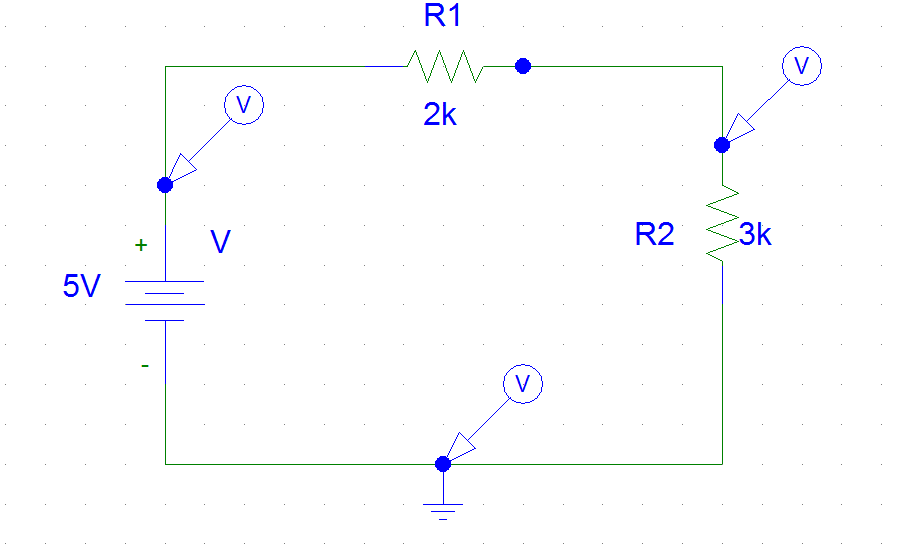
\includegraphics[width=11cm,height=7cm]{Img/dc_dos_resis.png}\\
		
		\noindent A este circuito se le realizaron los análisis transient y bias point detail obteniendo las siguientes gráficas de salida.\\
		
		\noindent En el análisis transient:\\
		
		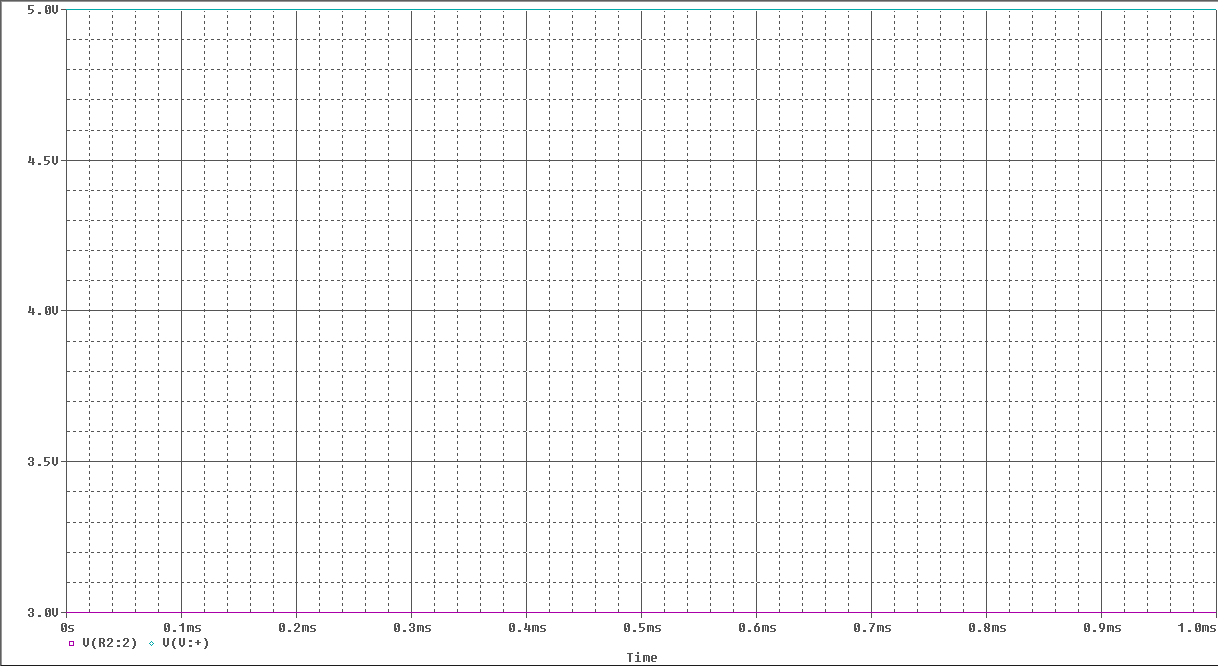
\includegraphics[width=11cm,height=7cm]{Img/Fuente_DC_y_dos_resistencias.png}
		
		\newpage
		 
		\noindent Y en el análisis bias point detail, se obtuvo:\\
		
		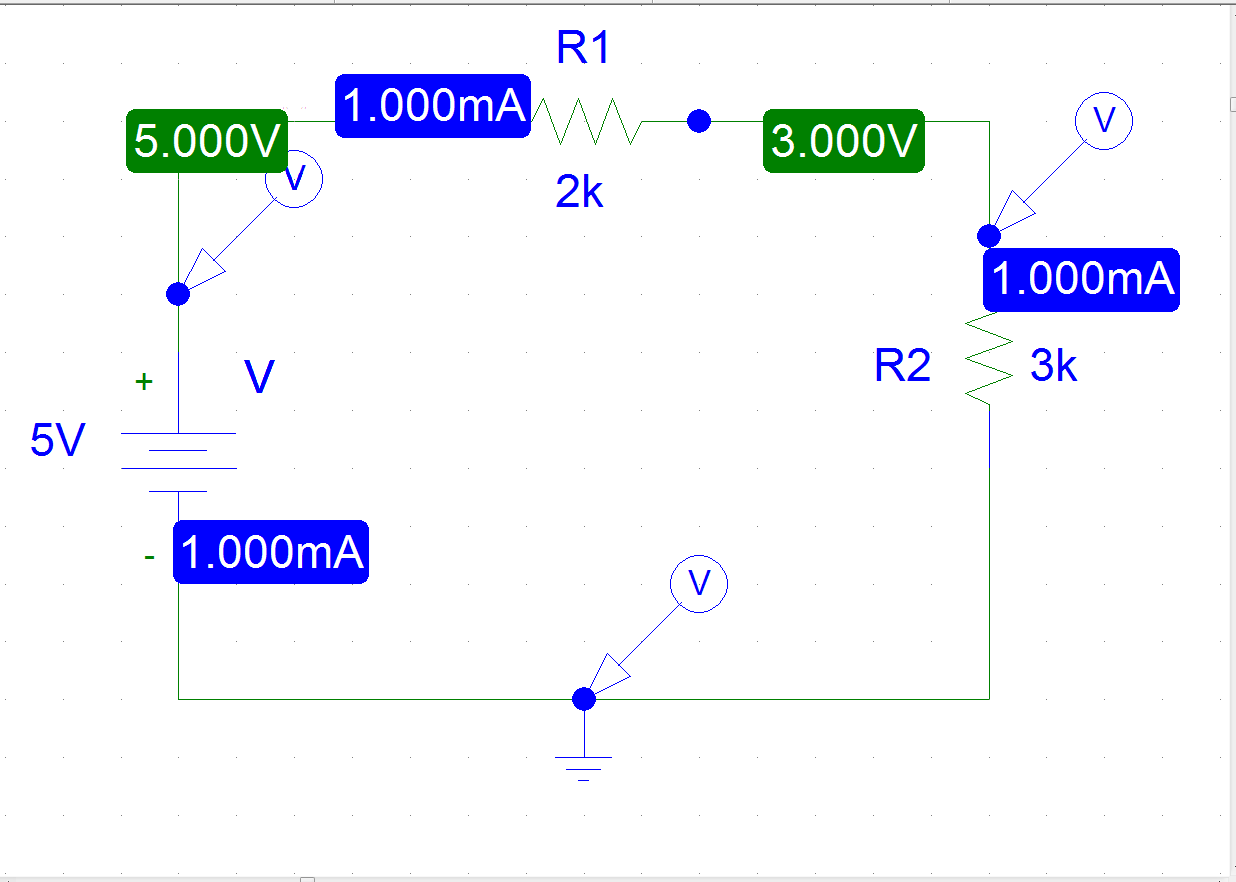
\includegraphics[width=11cm,height=7cm]{Img/Fuente_DC_y_dos_resistencias_Bias_analisis.png}\\
		
		\item \textbf{Circuito 2}- Corresponde a la figura 2.1.b\\ 
		
		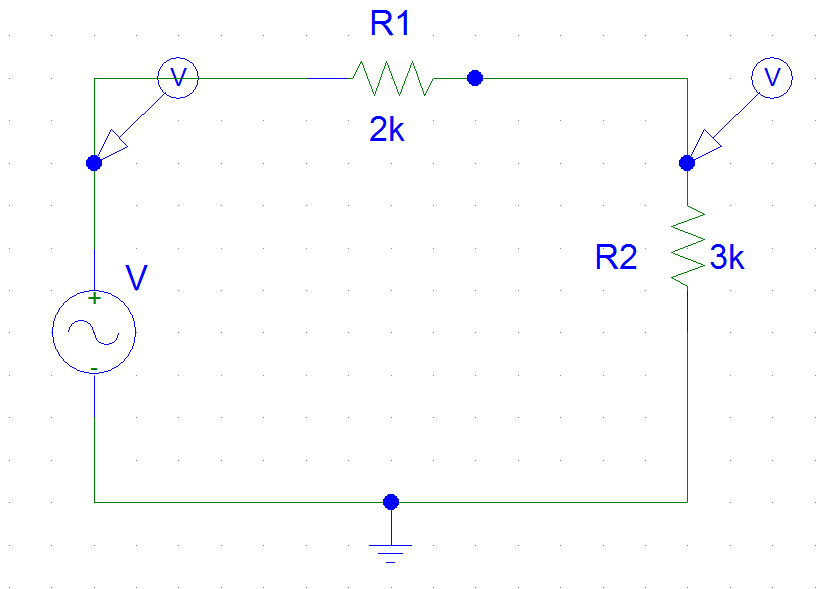
\includegraphics[width=11cm,height=7cm]{Img/ac_dos_resis.png}\\
		
		\noindent En este circuito sólo se aplicó el análisis transient, de donde se obtuvo:\\
		
		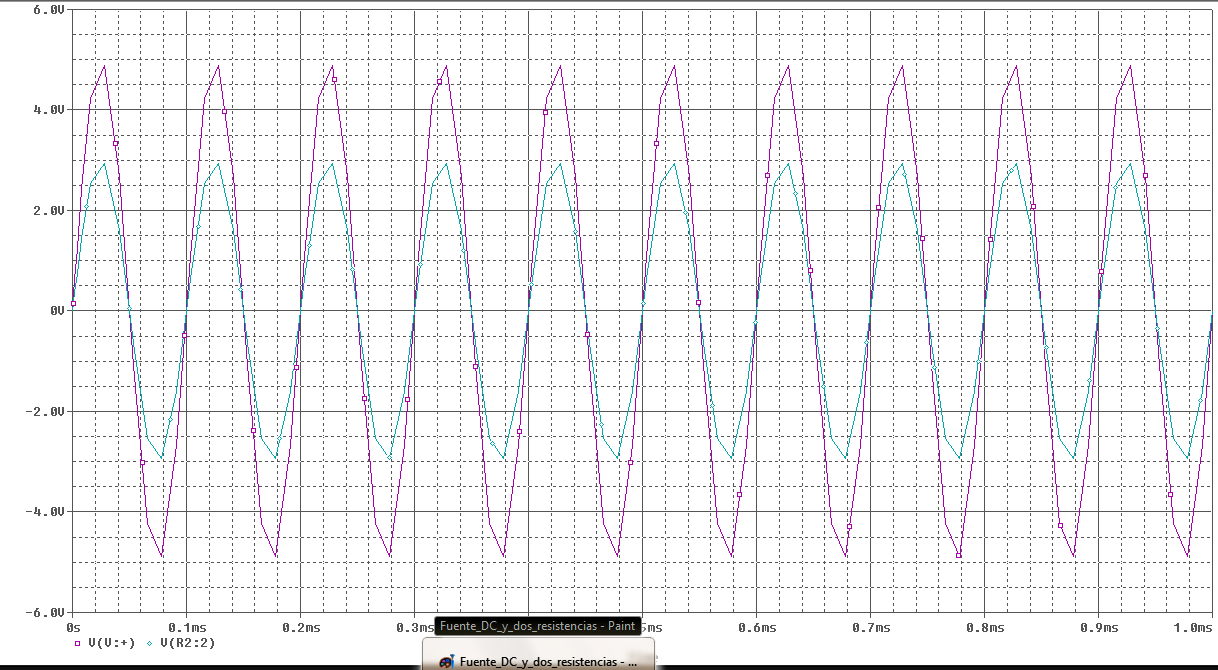
\includegraphics[width=11cm,height=7cm]{Img/Fuente_AC_y_dos_resistencias.png}\\
		
		\item \textbf{Circuito 3}- Corresponde a la figura 2.2.a\\ 
		
		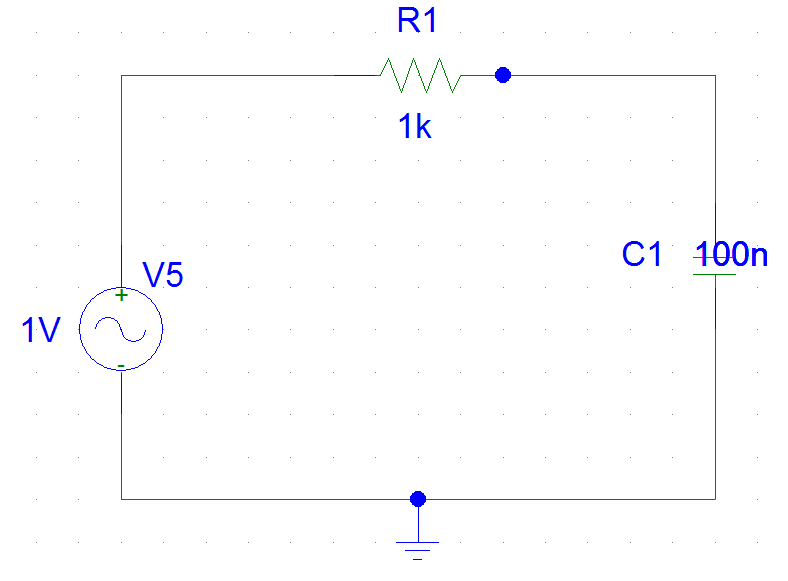
\includegraphics[width=11cm,height=7cm]{Img/ac_rc.png}\\
		
		\noindent Sobre este circuito se realizó un análisis transient, un análisis ac sweep y otro ac sweep sustituyendo la fuente por una de onda cuadrada.
		
		\noindent Transient\\
		
		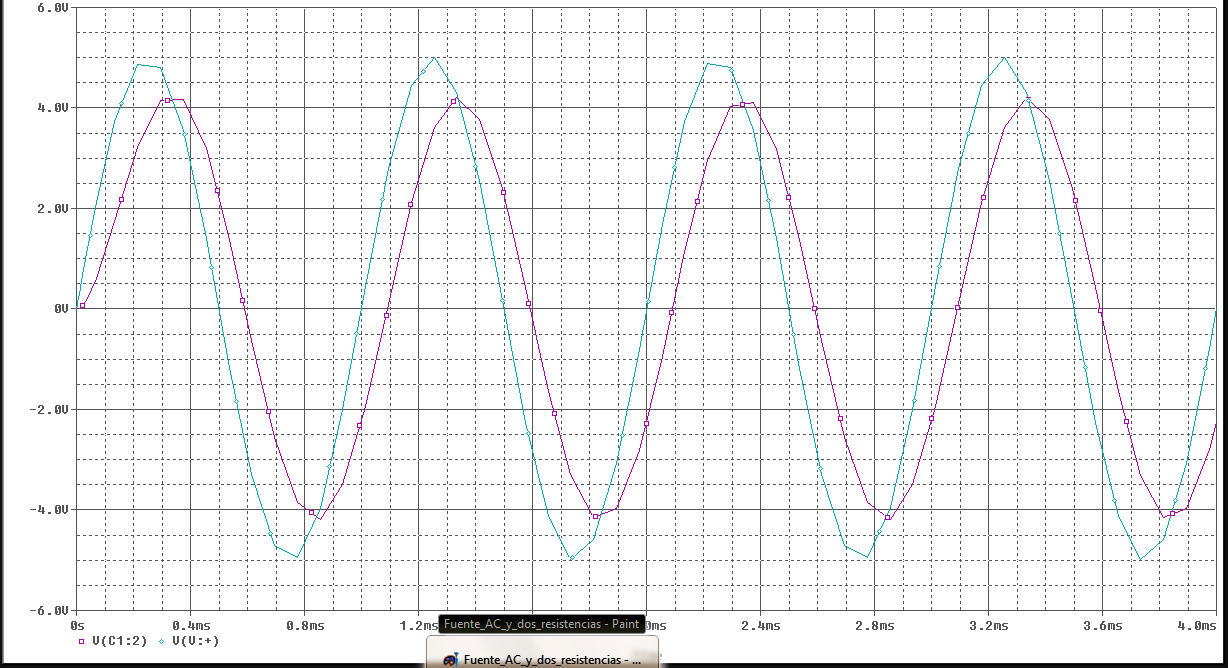
\includegraphics[width=11cm,height=7cm]{Img/Fuente_AC_RC.png}\\
		
		\noindent AC Sweep\\
		
		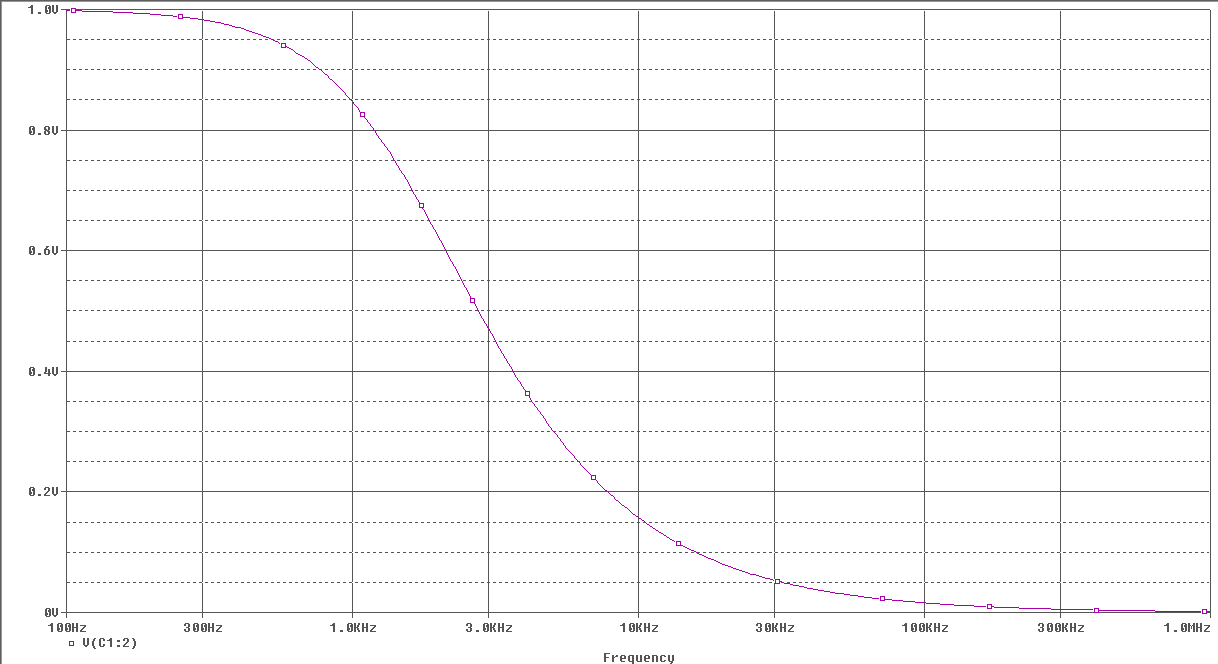
\includegraphics[width=11cm,height=7cm]{Img/Fuente_AC_RC_AC_sweep.png}\\
		
		\newpage 
		
		\noindent AC Sweep Vpulse\\
		
		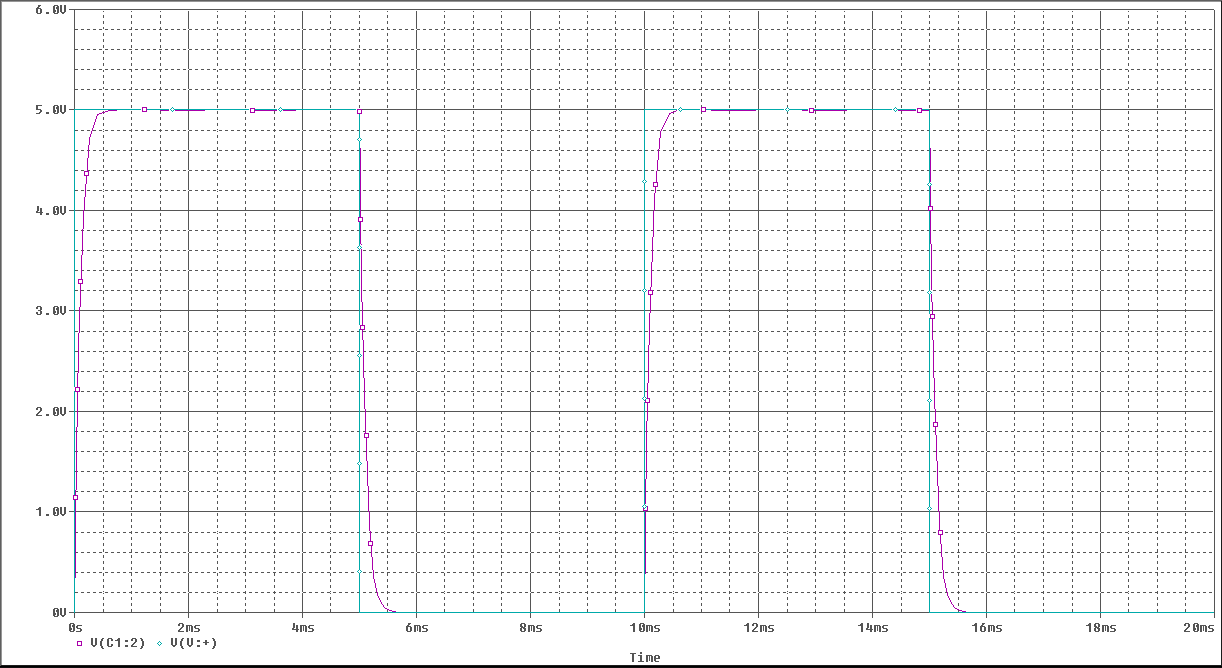
\includegraphics[width=11cm,height=7cm]{Img/Fuente_AC_RC_Vpulse}\\
		
		\item \textbf{Circuito 4}- Corresponde a la figura 2.2.b\\ 
		
		\noindent Es $L_2 = 100mH$ pero se nos pasó acomodar el display.\\
		
		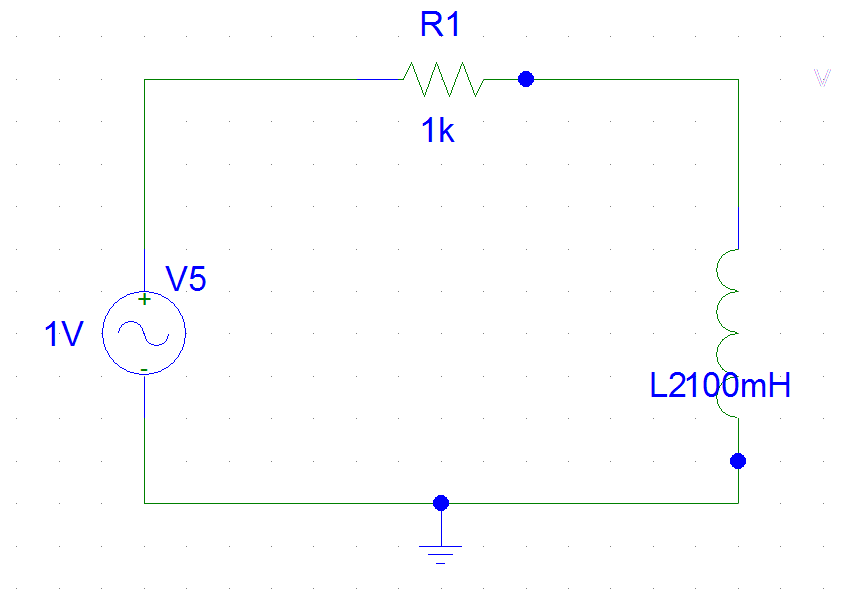
\includegraphics[width=11cm,height=7cm]{Img/ac_rl}\\
		
		\noindent Para este circuito también se hicieron los análisis transient, ac sweep y otro ac sweep con una fuente de onda cuadrada, quedando:
		
		\newpage
		
		\noindent Transient\\
		
		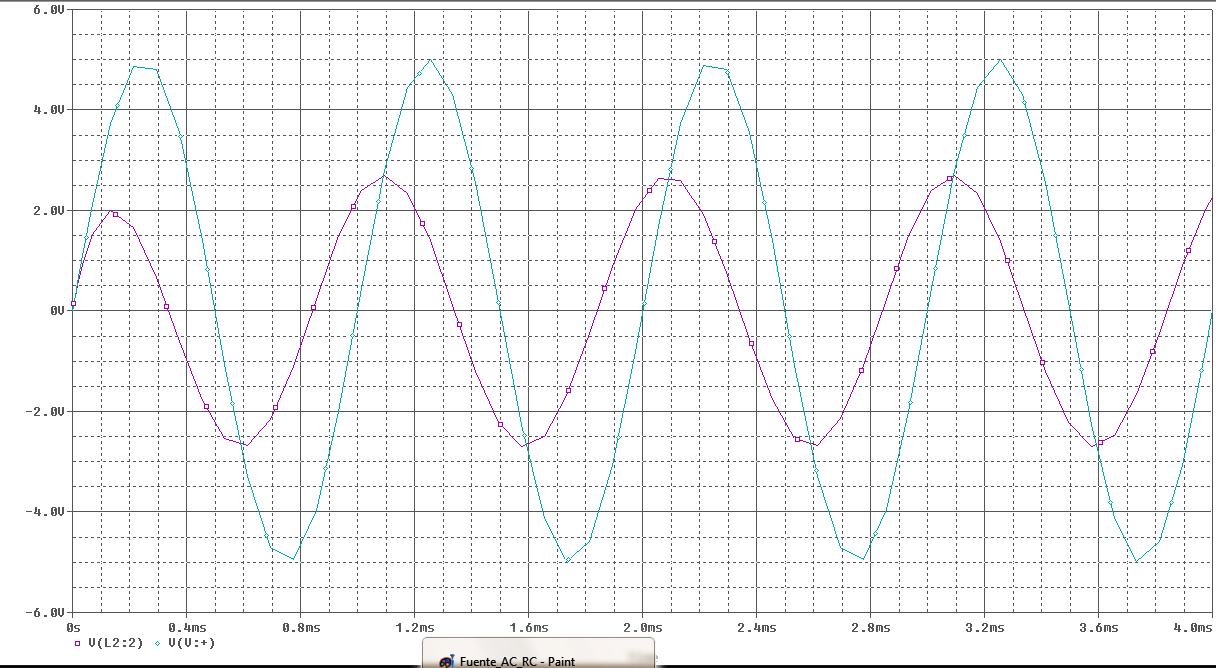
\includegraphics[width=11cm,height=7cm]{Img/Fuente_AC_RL}
		
		\noindent AC Sweep\\
		
		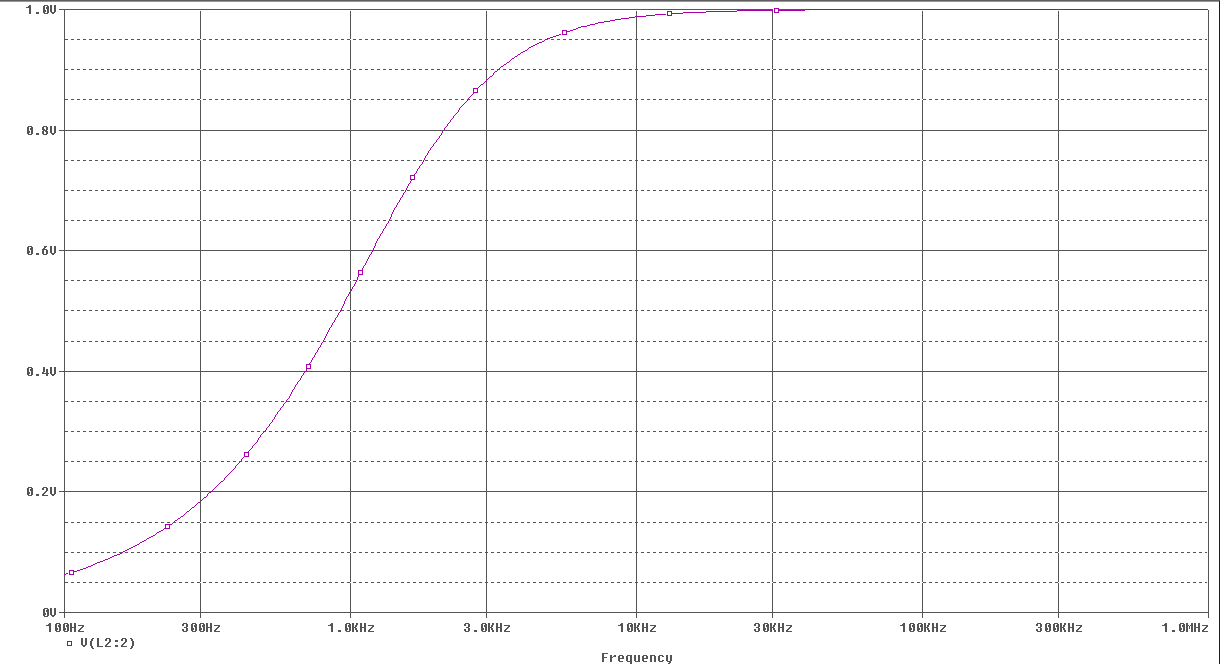
\includegraphics[width=11cm,height=7cm]{Img/Fuente_AC_RL_AC_sweep}
		
		\newpage
		
		\noindent AC Sweep Vpulse\\
		
		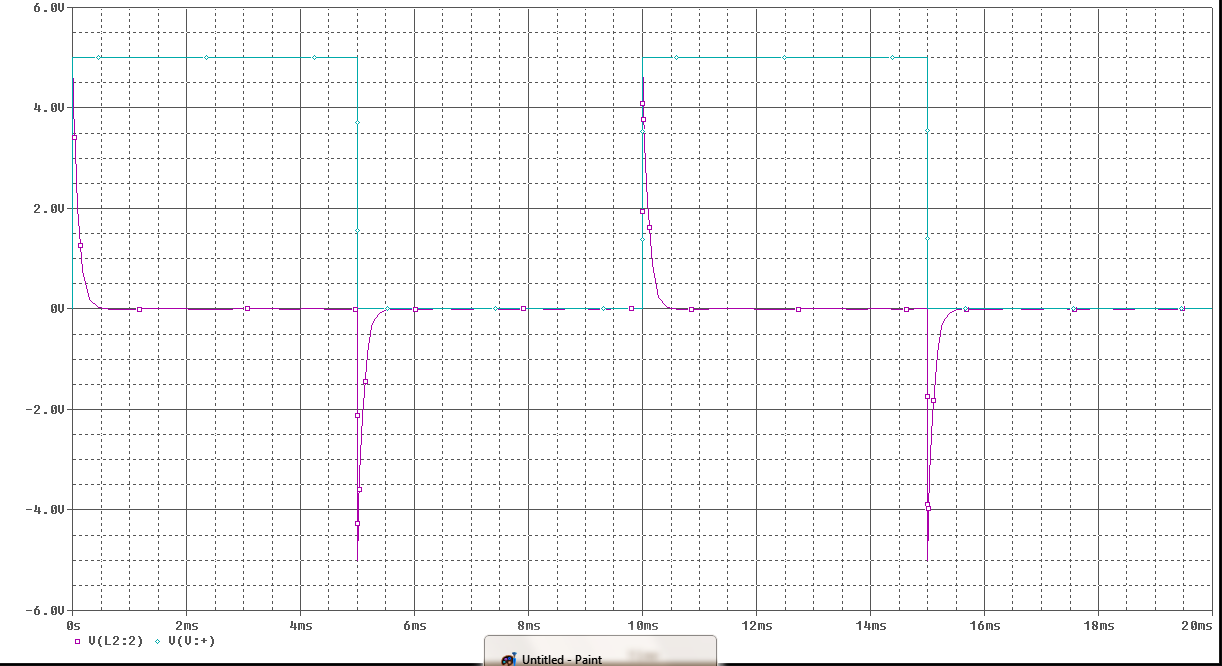
\includegraphics[width=11cm,height=7cm]{Img/Fuente_AC_RL_Vpulse}\\
		
		\item \textbf{Circuito 5}- Corresponde a la figura 2.3\\ 
		
		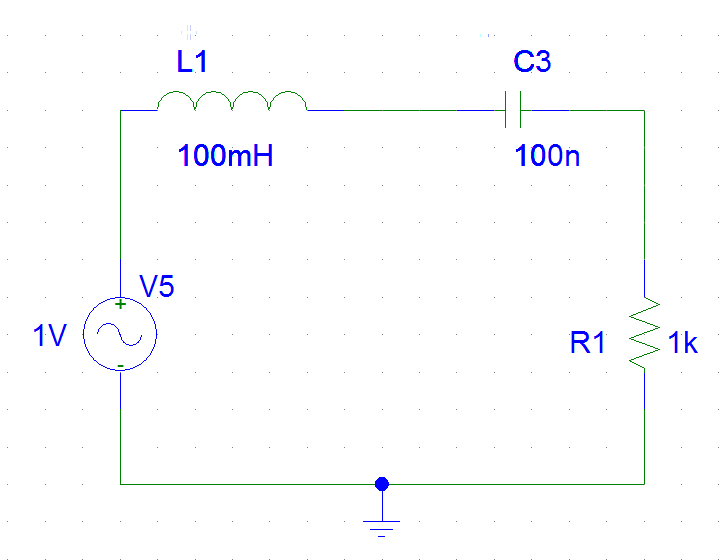
\includegraphics[width=11cm,height=7cm]{Img/ac_rlc}\\
		
		\noindent En este circuito se hicieron cuatro análisis ac sweep, uno sobre la resistencia, sobre la inductancia, sobre la capacitancia y uno sobre la inductancia y la capacitancia en serie. Resultando en:
		
		\newpage
		
		\noindent AC Sweep sobre la resistencia\\
		
		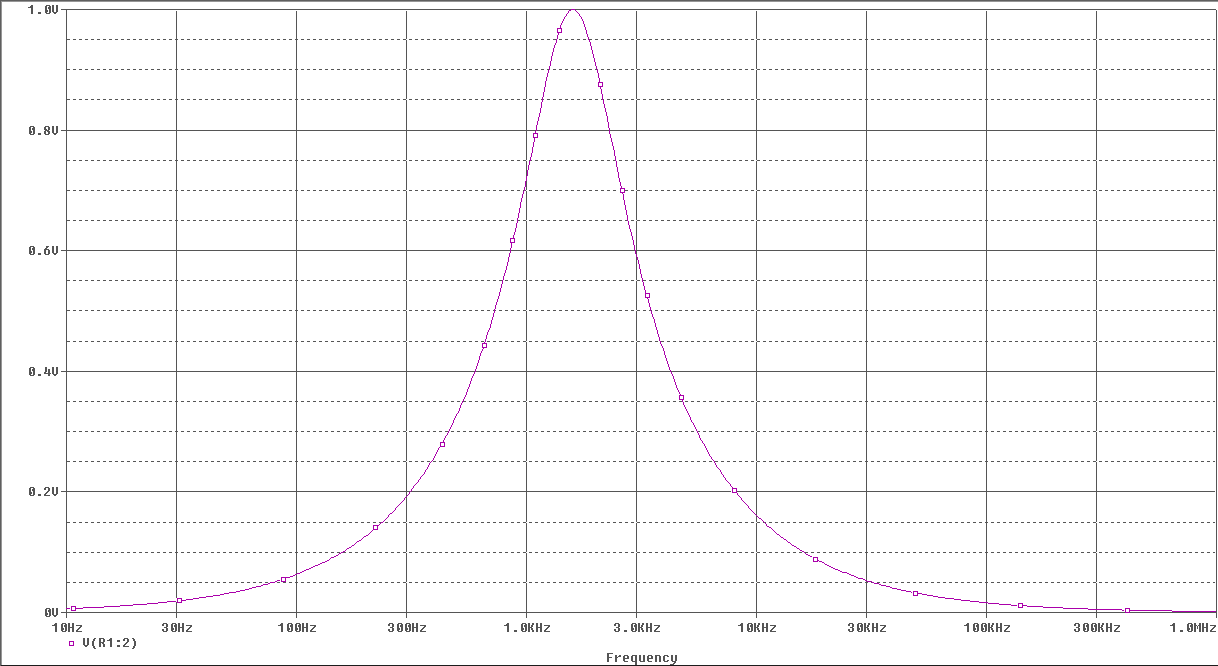
\includegraphics[width=11cm,height=7cm]{Img/Fuente_AC_RLC_AC_Sweep_Resistencia}\\
		
		\noindent AC Sweep sobre la inductancia\\
		
		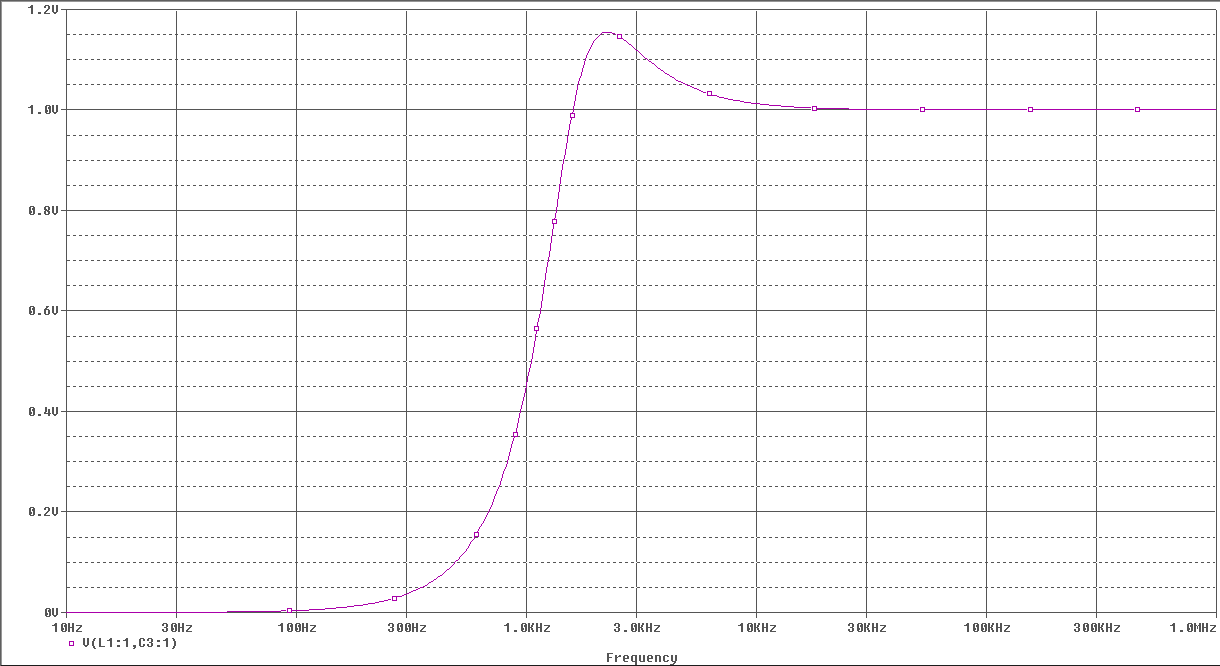
\includegraphics[width=11cm,height=7cm]{Img/Fuente_AC_RLC_AC_Sweep_L}
		
		\newpage
		
		\noindent AC Sweep sobre la capacitancia\\
		
		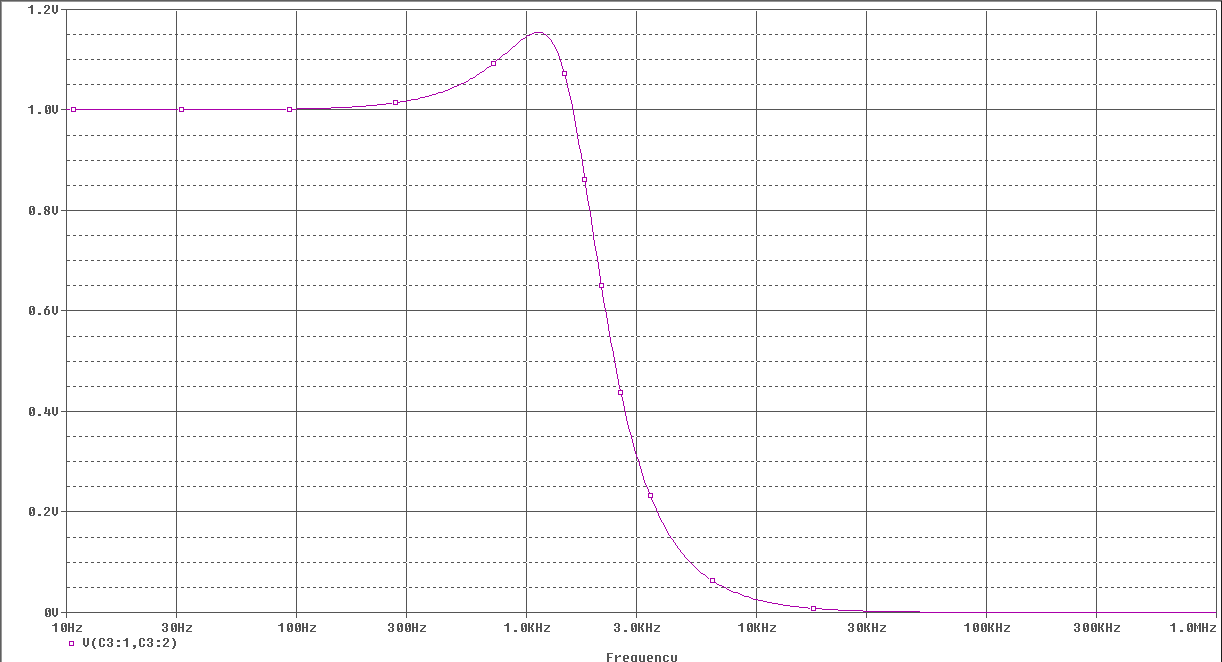
\includegraphics[width=11cm,height=7cm]{Img/Fuente_AC_RLC_AC_Sweep_C}\\
		
		\noindent AC Sweep sobre la inductancia y la capacitancia en serie\\
		
		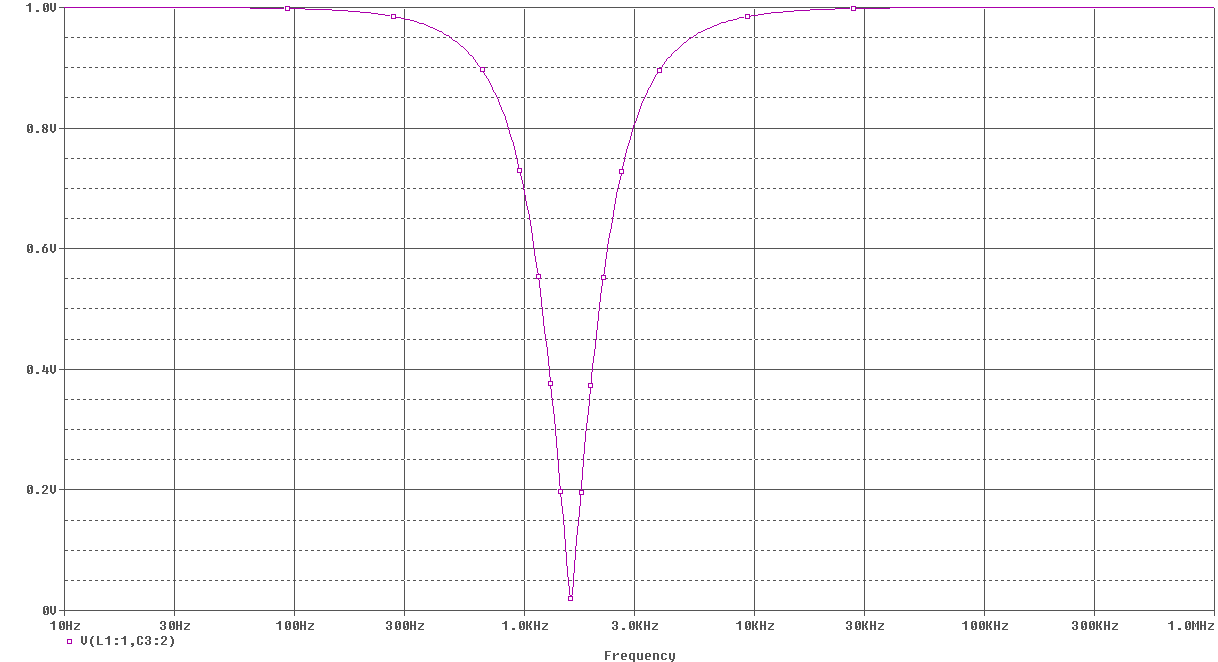
\includegraphics[width=11cm,height=7cm]{Img/Fuente_AC_RLC_AC_Sweep_LC}\\
		
		\item \textbf{Circuito 6}- Corresponde a la figura 2.4 en configuración estrella-estrella\\
		
		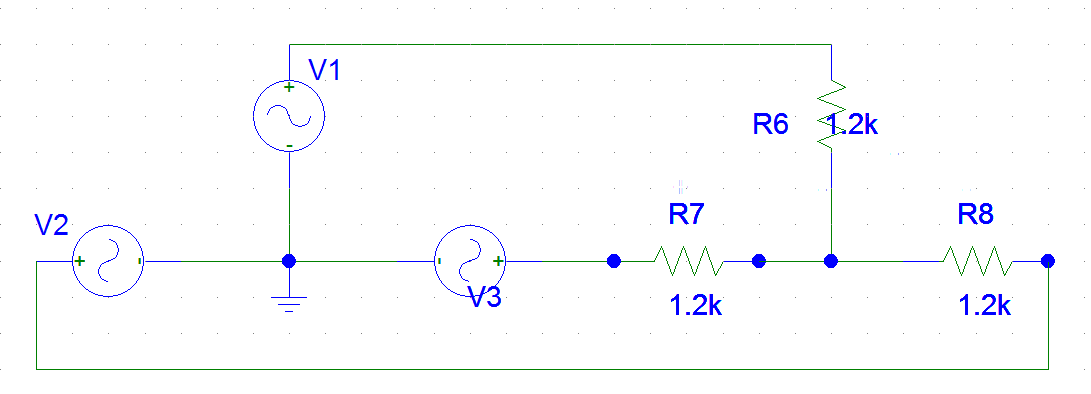
\includegraphics[width=11cm,height=7cm]{Img/trifas_str_str}\\
		
		\noindent Este circuito se sometió a dos análisis transient, uno para las fuentes y otro para las resistencias ambos análisis resultaron en la misma gráfica.\\
		
		\noindent Análisis sobre las fuentes\\
		
		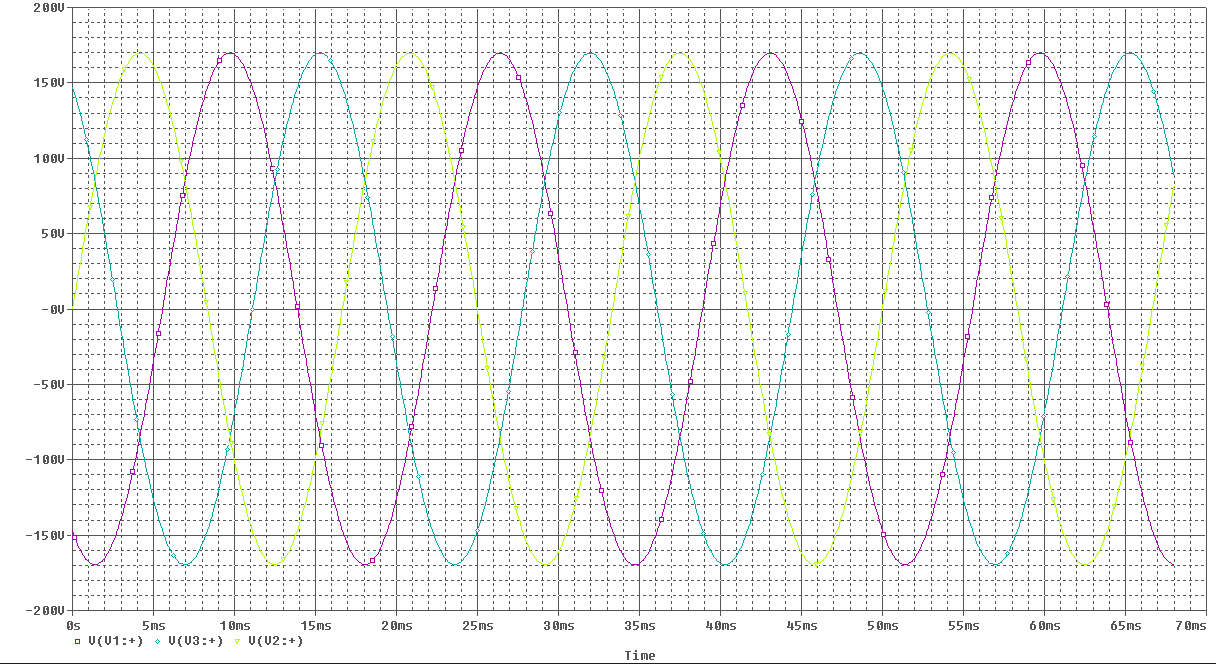
\includegraphics[width=11cm,height=7cm]{Img/Circuito_trifasico_estrella_delta}\\
		
		\noindent Análisis sobre las resistencias\\
		
		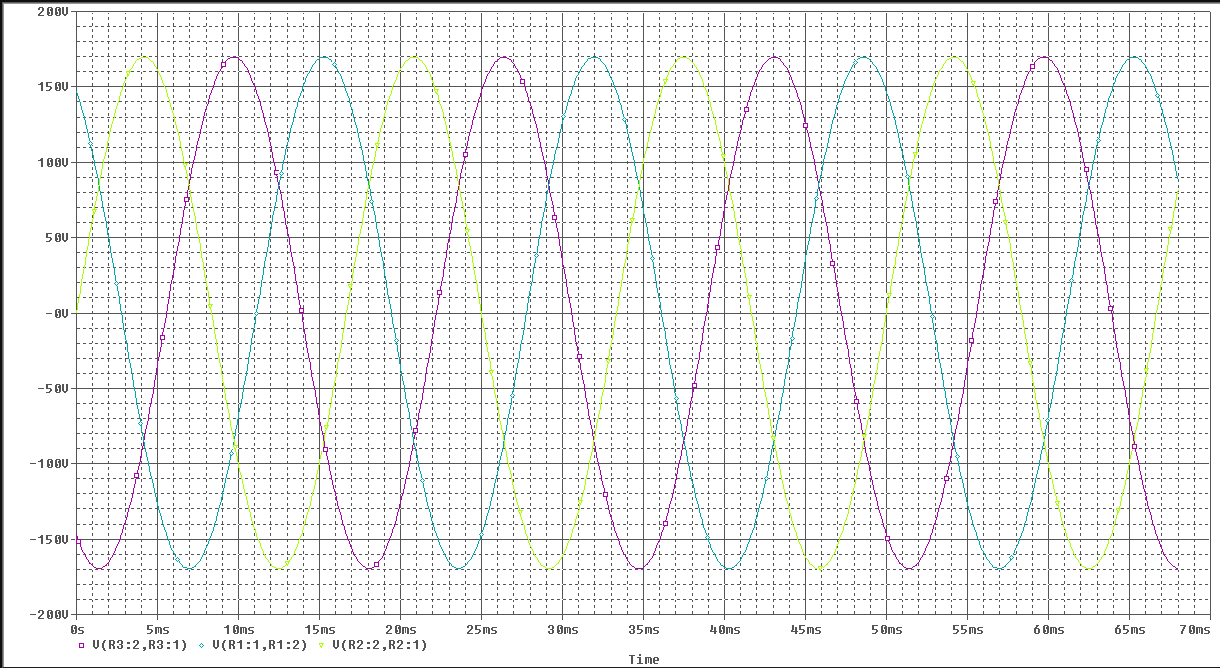
\includegraphics[width=11cm,height=7cm]{Img/circ_trifas_estr_estr_resistencias}\\
		
		\item \textbf{Circuito 7}- Corresponde a la figura 2.4 en configuración estrella-delta\\
		
		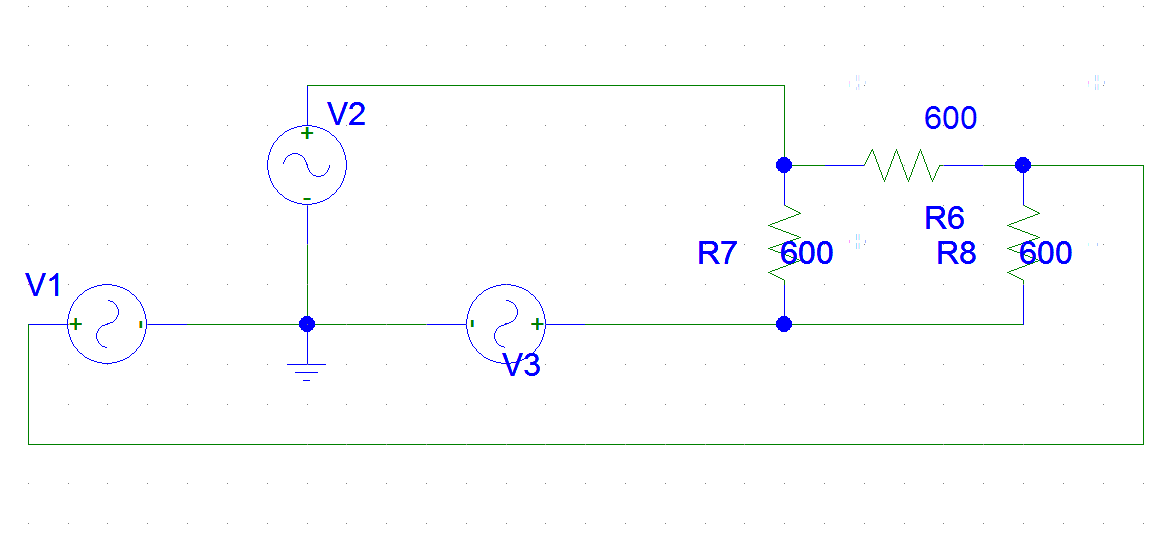
\includegraphics[width=11cm,height=7cm]{Img/trifas_str_dlt}\\
		
		\noindent Sobre esta configuración se aplicó el mismo análisis que en el anterior.\\
		
		\noindent Análisis sobre las fuentes\\
		
		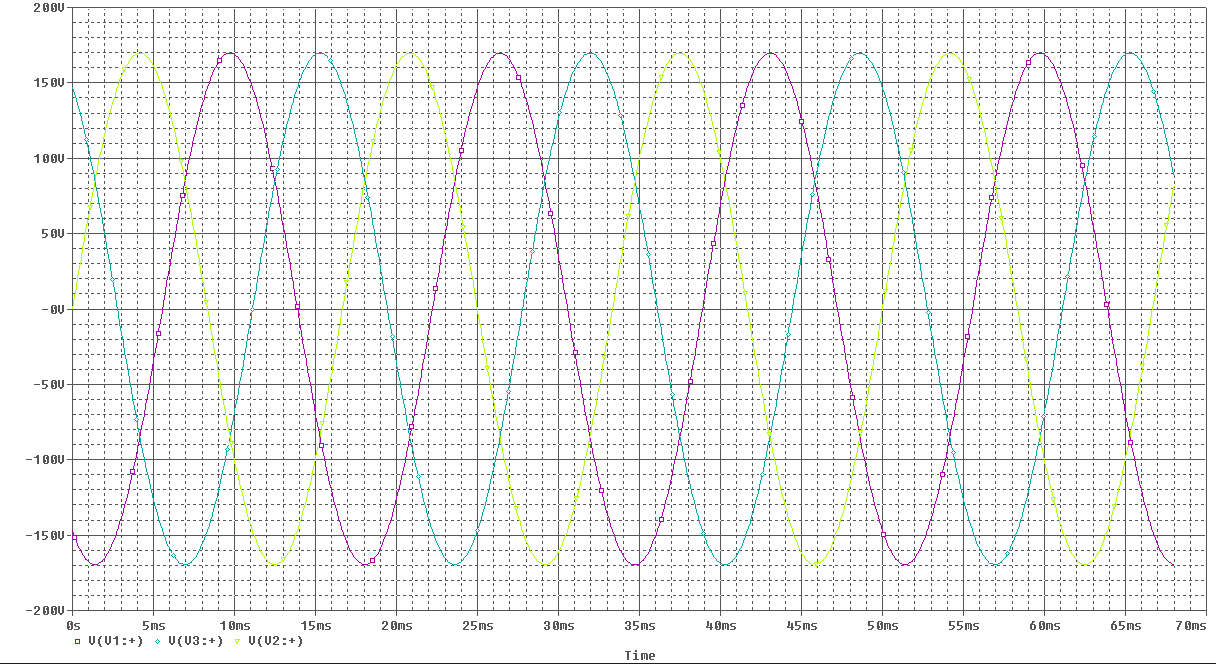
\includegraphics[width=11cm,height=7cm]{Img/Circuito_trifasico_estrella_delta}\\
		
		\noindent Análisis sobre las resistencias\\
		
		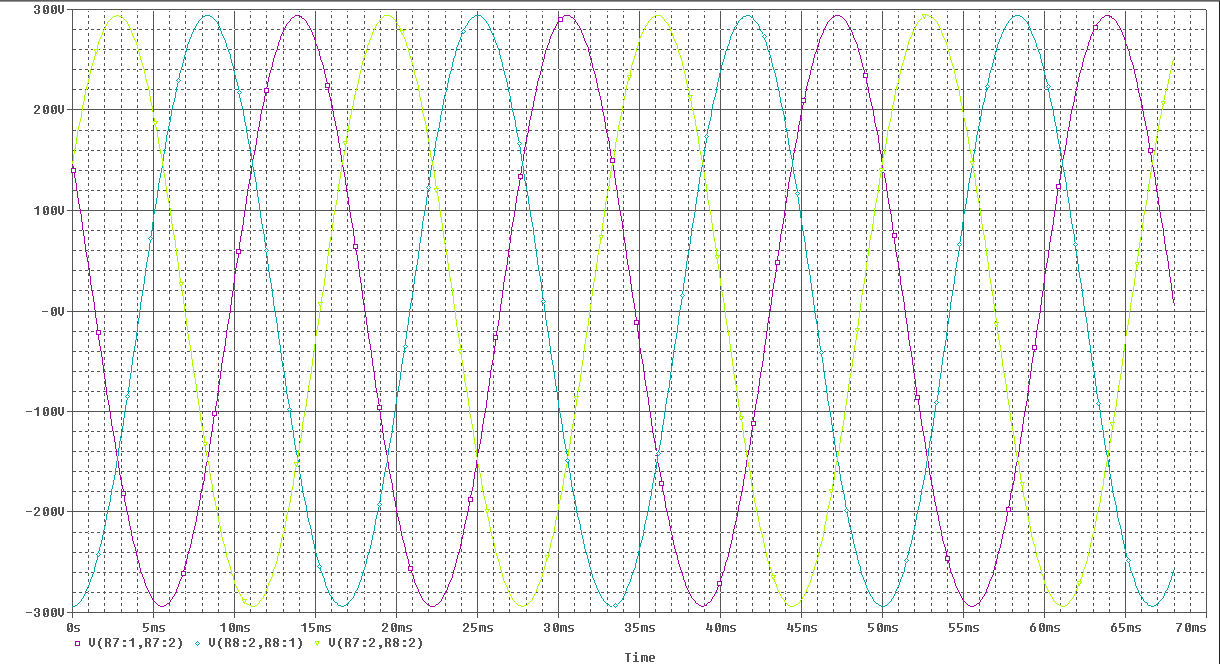
\includegraphics[width=11cm,height=7cm]{Img/Circ_trifas_estr_delta_resist}
		
		\newpage
		
		\item \textbf{Circuito 8}- Corresponde a la figura 2.5\\
		
		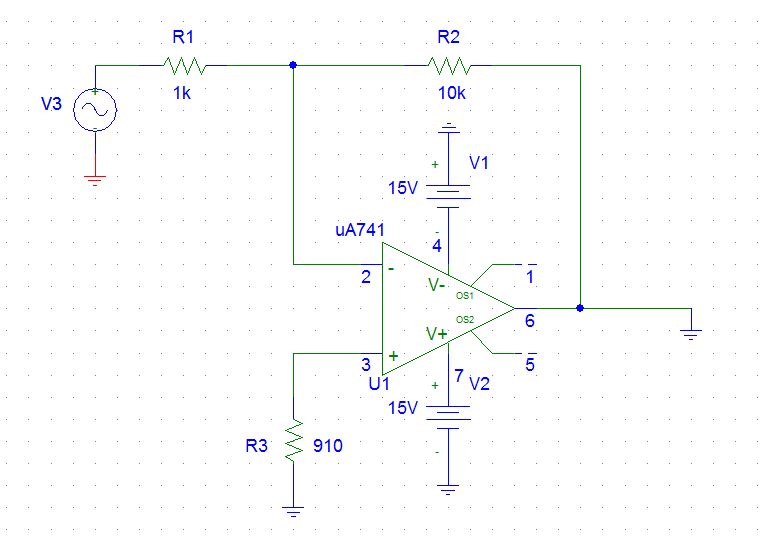
\includegraphics[width=11cm,height=7cm]{Img/opam_ua741}\\

		\noindent En este circuito se realizaron tres configuraciones donde se cambiaba la fuente conectada a $R_1$, en el primero se conectó una fuente constante y se realizó un bias point detail, en el segundo se usó una fuente vsin y se hizo un análisis transient, finalmente en el tercero se usó una fuente vac y se le realizó un análisis ac sweep.\\
		
		\noindent Fuente DC. Análisis Bias Point Detail\\
		
		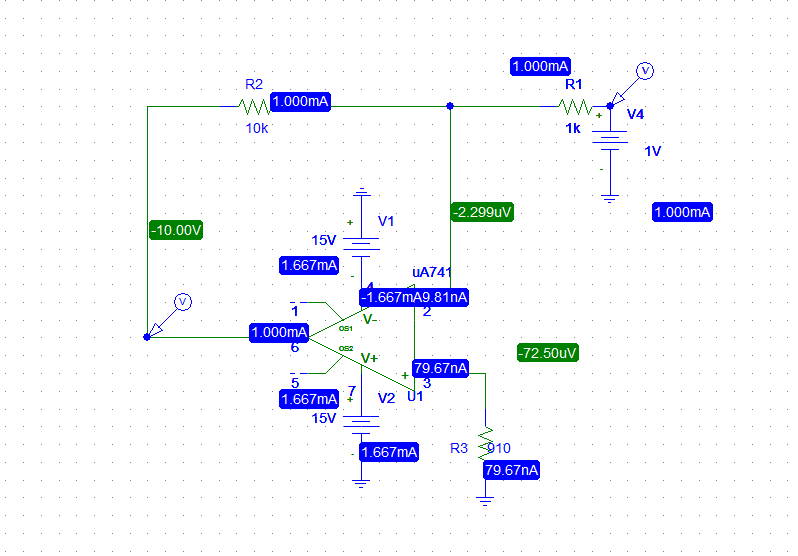
\includegraphics[width=11cm,height=7cm]{Img/opam_ua741_bias_analisis_DC}\\
		
		\newpage
		
		\noindent Fuente AC. Análisis Transient\\
		
		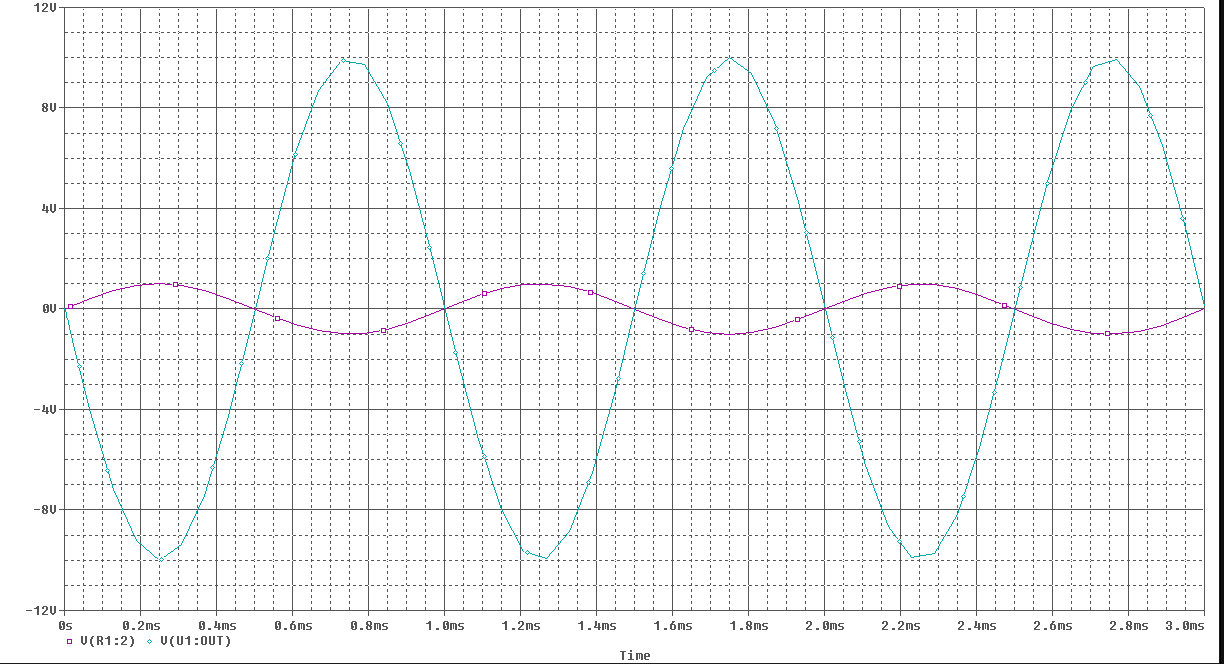
\includegraphics[width=11cm,height=7cm]{Img/opam_ua741_transient_AC}\\
		
		\noindent Fuente AC. Análisis AC Sweep\\
		
		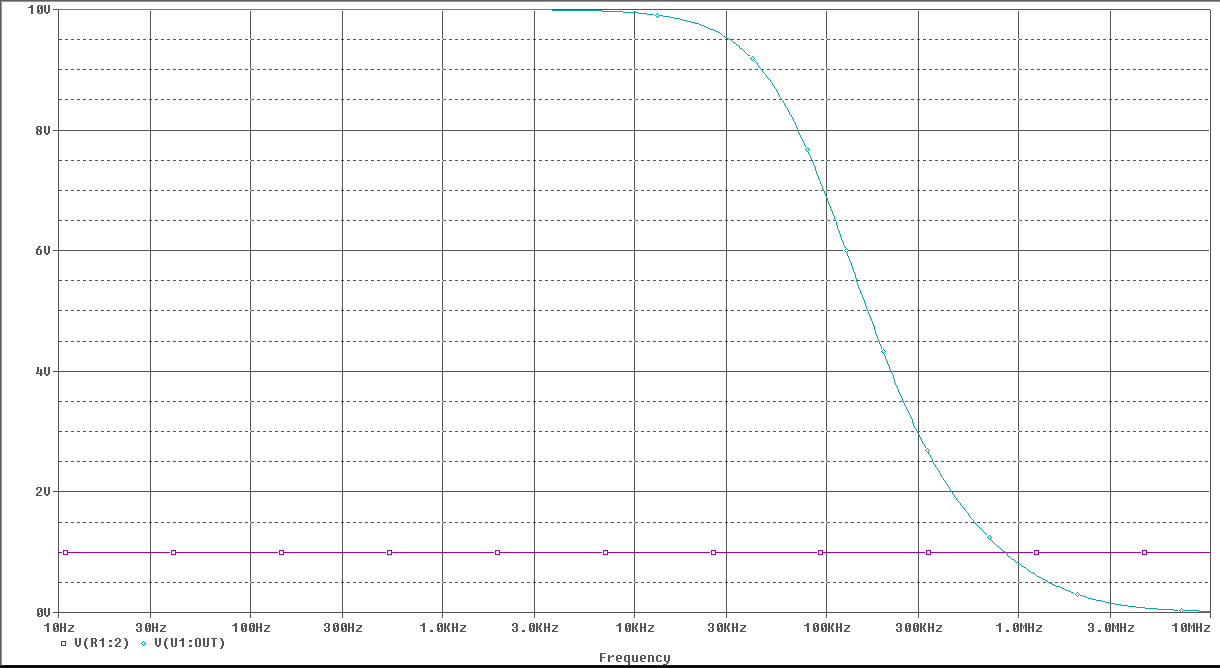
\includegraphics[width=11cm,height=7cm]{Img/opam_ua741_AC_sweep}\\
		
		\newpage
		
		\item \textbf{Circuito 9}- Corresponde a la figura 2.6\\
		
		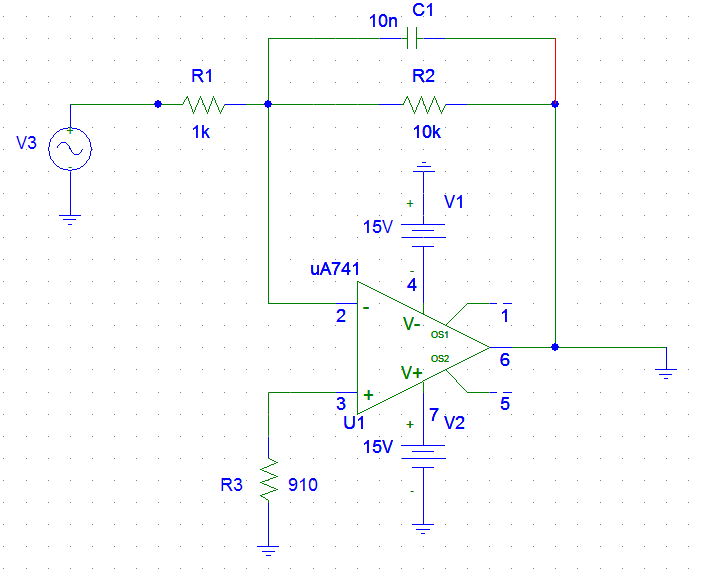
\includegraphics[width=11cm,height=7cm]{Img/opam_ua741_pasa_bajo_act}\\
		
		\noindent Para esta configuración se aplicó un análisis ac sweep que resultó en:\\
		
		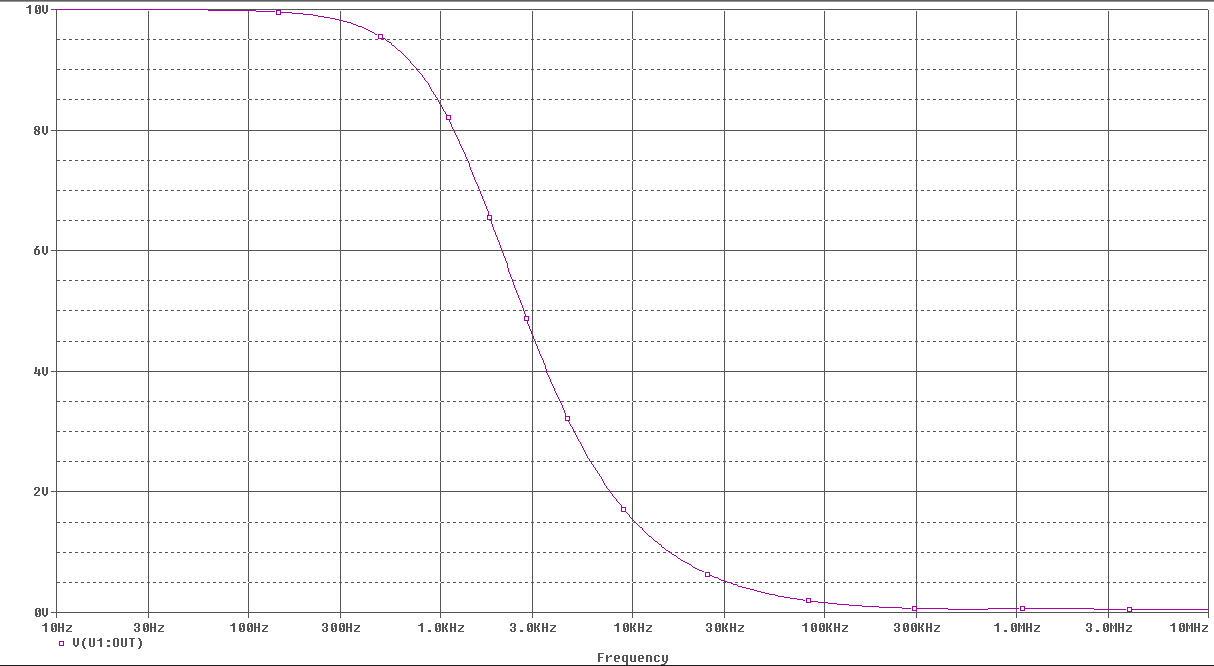
\includegraphics[width=11cm,height=7cm]{Img/filtro_pasa_bajo_activo}\\
		
		\newpage
		
		\item \textbf{Circuito 10}- Corresponde a la figura 2.7\\
		
		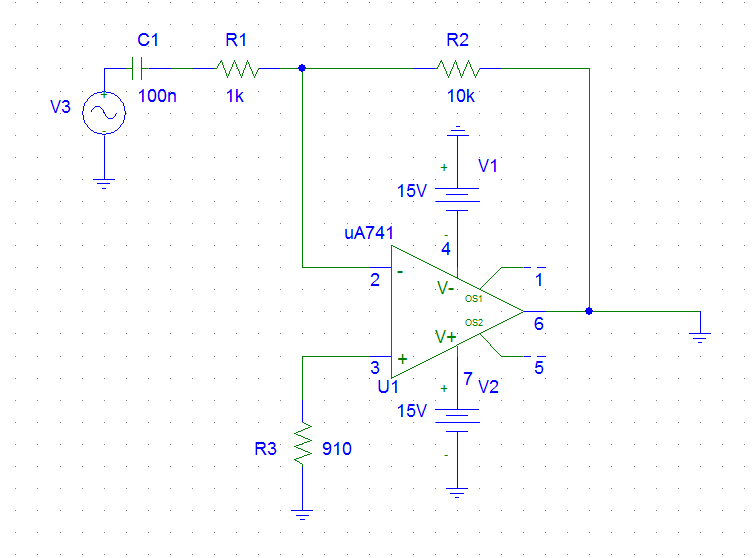
\includegraphics[width=11cm,height=7cm]{Img/opam_ua741_pasa_alto_act}\\
		
		\noindent En este circuito también se implementó un ac sweep:\\
		
		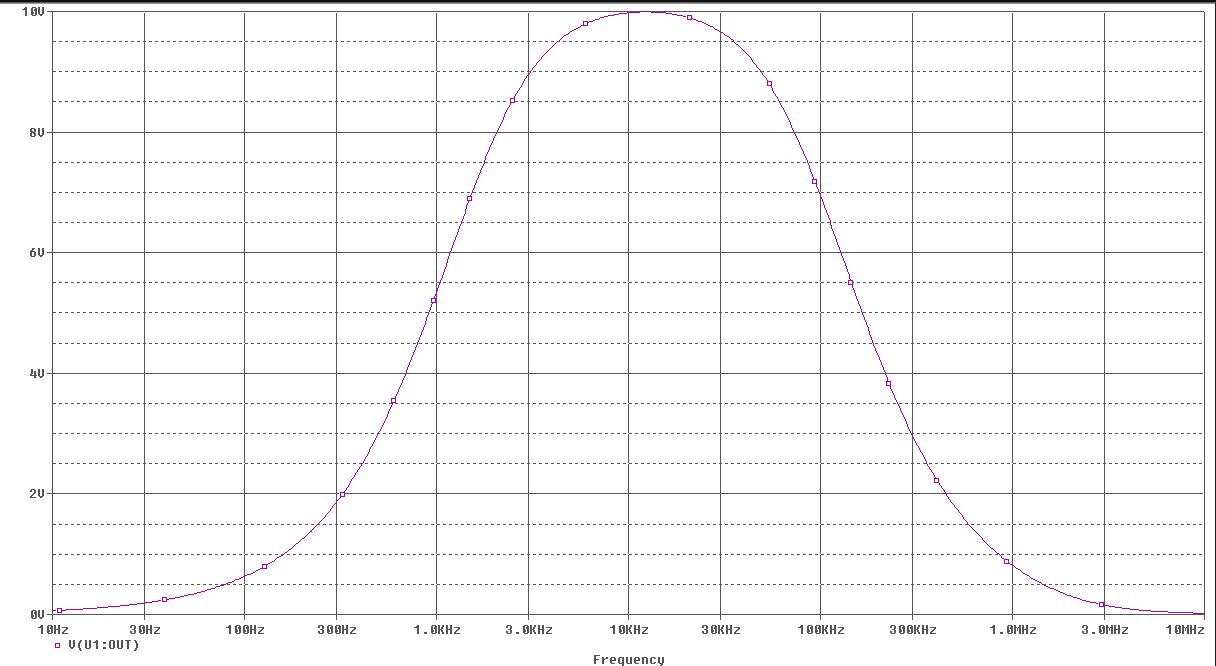
\includegraphics[width=11cm,height=7cm]{Img/filtro_pasa_alto_activo}\\
		
	\end{itemize}
	
	\newpage
	
	\begin{center}
		\textbf{\large ANÁLISIS DE RESULTADOS}\\
	\end{center}
	
	\renewcommand{\theenumi}{\alph{enumi}} %Letras minúsculas 
	
	\begin{enumerate}
		\item Los valores de voltaje DC sobre las dos resistencias del circuito 2.1.a\\
		
		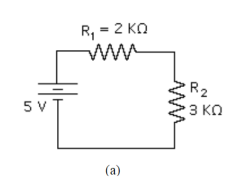
\includegraphics{Img/2_1_a}
		
		\noindent Acá tendremos las siguientes relaciones mediante divisor de voltajes:\\
		
		\begin{equation}
			\notag V_1 = \frac{R_1}{R_1 + R_2} V_f = \frac{2k\Omega}{5k\Omega}(5V) = 2V
		\end{equation}
	
		\begin{equation}
			\notag V_2 = \frac{R_2}{R_1 + R_2} V_f = \frac{3k\Omega}{5k\Omega}(5V) = 3V
		\end{equation}
	
		\noindent En el gráfico se aprecia que la fuente se mantiene en el valor de $5V$, la resistencia $R_2$ sobre la cual se midió el voltaje tiene $3V$ y la tierra por supuesto se encuentra a $0V$.
		
		\item Los valores de voltaje pico sobre las dos resistencias del circuito 2.1.b\\
		
		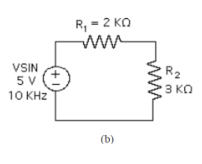
\includegraphics{Img/2_1_b}
		
		\noindent En este caso, el voltaje pico de la fuente oscila entre $5V$ y $-5V$, mientras que el voltaje pico sobre $R_2$ oscila entre $3V$ y $-3V$, esto sucede debido a que el voltaje no es constante en el tiempo, sin embargo, en el dominio fasorial, se puede evidenciar que mediante divisor de voltaje se obtienen esos valores pico.
		
		\item Los valores de voltaje pico sobre la resistencia $V_{R_p}$, el
		voltaje pico sobre el condensador $V_{C_p}$ y el valor de la
		frecuencia de corte del filtro pasa bajo presentado en la figura 2.2.a
		
		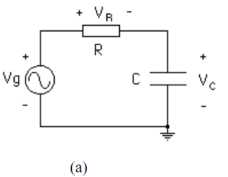
\includegraphics{Img/2_2_a}\\
		
		\noindent Para esta configuración se aplicarán las fórmulas proporcionadas en las instrucciones para la realización del informe.\\
		
		\begin{equation}
			\notag V_{R_p} = \frac{R}{\sqrt{R^2 + (\frac{1}{2\pi f C})^2}}V_p = \frac{1k\Omega}{\sqrt{1k\Omega ^2 + \Big (\frac{1}{2\pi (1kHz) (100nF)}\Big)^2}}(5V) = 2.66V
		\end{equation}
		\\
		
		\begin{equation}
			\notag V_{C_p} = \frac{\frac{1}{2 \pi f C}}{\sqrt{R^2 + (\frac{1}{2\pi f C})^2}}V_p = \frac{\frac{5V}{2\pi (1kHz) (100nF)}}{\sqrt{1k\Omega ^2 + \Big (\frac{1}{2\pi (1kHz) (100nF)}\Big)^2}} = 4.23V
		\end{equation}
		
		\noindent La gráfica no tiene sufiente precisión para determinar los valores exactos, sin embargo, se puede apreciar que los valores está, cercanos a los valores arrojados por la gráfica.\\
		
		\noindent La frecuencia de corte se determina mediante:\\
		
		\begin{equation}
			\notag f_C = \Big(\frac{1}{2\pi}\Big)\Big(\frac{1}{RC}\Big) = \Big(\frac{1}{2\pi (1k\Omega)(100nF)}\Big) = 1591.55Hz
		\end{equation}\\
		
		\noindent En la gráfica del análisis AC sweep se ve claramente como después de los $1kHz$ el voltaje baja al $70\%$, es decir, elimina los voltajes a frecuencias muy altas.\\
		
		\item Los valores de voltaje pico sobre la resistencia $V_{R_p}$, el voltaje pico sobre la inductancia $V_{L_p}$ y el valor de la frecuencia de corte del filtro alto RL presentado en la figura 2.2.b
		
		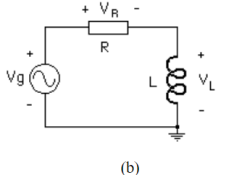
\includegraphics{Img/2_2_b}\\
		
		\noindent Nuevamente aplicamos las fórmulas propuestas en el documento donde se explica el informe:\\
		
		\begin{equation}
			\notag V_{R_p} = \frac{R}{\sqrt{R^2 + (2\pi f L)^2}}V_p = \frac{1k\Omega}{\sqrt{1k\Omega ^2 + \Big (2\pi (1kHz) (100mH)\Big)^2}}(5V) = 4.23V
		\end{equation}\\
	
		\begin{equation}
			\notag V_{L_p} = \frac{R}{\sqrt{R^2 + (2\pi f L)^2}}V_p = \frac{2\pi (1kHz) (100mH)}{\sqrt{1k\Omega ^2 + \Big (2\pi (1kHz) (100mH)\Big)^2}}(5V) = 2.66V
		\end{equation}\\
	
		\noindent Para la frecuencia se tiene la expresión:\\
		
		\begin{equation}
			\notag f_L = \Big(\frac{1}{2\pi}\Big)\Big(\frac{R}{L}\Big) = \Big(\frac{(1k\Omega)}{2\pi (100nF)}\Big) = 1591.55Hz
		\end{equation}\\
	
		\noindent El resultado es análogo al circuito anterior, sin embargo, en la gráfica esta vez se evidencia que la frecuencia de corte muestra el aumento hasta el $70\%$ del voltaje, es decir, el filtro elimina los voltajes a bajas frecuencias.\\
		
		\item Las constantes de tiempo del circuito RC ($t = RC$) y del circuito RL ($t = L/R$):\\
		
		\begin{itemize}
			\item Circuito RC:\\
			
			\begin{equation}
				\notag \tau = RC = (1k\Omega)(100nF) = 0.1ms
			\end{equation}\\
		
			\noindent En la gráfica se puede evidenciar que para ese tiempo, la carga del condensador está a $\frac{1}{3}$ de su carga máxima, por lo que su diferencia de potencial seguirá aumentando hasta cargarse completamente, en un circuito de corriente contínua, al cargarse el condensador actuaría como circuito abierto, sin embargo, acá, al tratarse de corriente que oscila en dos direcciones, el condensador se carga y se descarga varias veces.\\
			
			\item Circuito RL:
			
			\begin{equation}
				\notag \tau = \frac{L}{R} = \frac{100mH}{1k\Omega} = 0.1ms
			\end{equation}\\
			
			\noindent Acá el resultado es análogo al anterior, la única diferencia es el comportamiento del inductor, es conocido que en corriente alterna el inductor evita el cambio brusco de la corriente, mientras que el capacitor regula el voltaje en este tipo de circuitos.\\
			
		\end{itemize}
		
		\item Frecuencia de resonancia del circuito RLC de la figura 2.3\\
		
		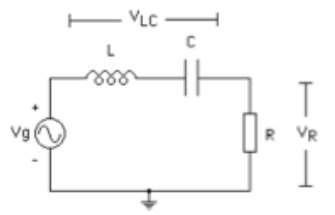
\includegraphics{Img/2_3}\\
		
		\noindent La ecuación propuesta para la frecuencia de resonancia es:\\
		
		\begin{equation}
			\notag f_r = \frac{1}{2\pi}\sqrt{\frac{1}{LC}} = \frac{1}{2\pi}\sqrt{\frac{1}{(100mH)(100nF)}} = 1591.55Hz
		\end{equation}\\
	
		\noindent En este circuito se puede apreciar que justo en la frecuencia de corte, la diferencia de potencial que circula es la máxima, es decir, sólo se da paso a voltajes en un determinado rango de frecuencias.\\
		
		\item La ganancia del amplificador inversor de la figura 2.5\\
		
		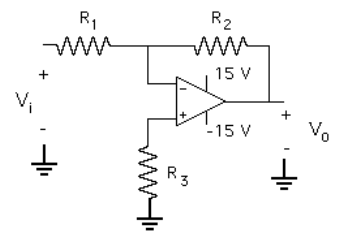
\includegraphics{Img/2_5}\\
		
		\noindent En el curso EC1251 se estudió que para un opam inversor, se cumple que:\\
		
		\begin{equation}
			\notag \frac{V_0}{V_i} = -\frac{R_2}{R_1} = -\frac{10k\Omega}{1k\Omega} = -10
		\end{equation}\\
	
		\noindent Dicho valor quedó corroborado ya que en el bias point detail $V_i = 1V$ y $V_0 = -10V$, lo cual confirma que el análisis mediante ecuaciones es correcto, aún más queda evidenciado en el análisis con corriente alterna, ya que los valores del voltaje para corriente directa serán los valores pico para alterna. En la gráfica de alterna e evidencia cómo el primer ciclo lleva a $V_0$ desde $0V$ hasta $-10V$ y el voltaje en $R_1$ de $0$ a $1V$, por supuesto, cabe a destacar que al ser corriente alterna, sus ciclos oscilan, cambiando el sentido de la corriente, por lo que hay puntos donde $V_0$ llega a $10V$.\\
		
		\noindent Para el AC sweep se evidencia el punto en el cual $V_0$ corta a $V_{R_1}$ y empieza el otro ciclo de carga.\\
		
		\item La frecuencia de corte del filtro pasa bajo activo de la figura 2.6\\
		
		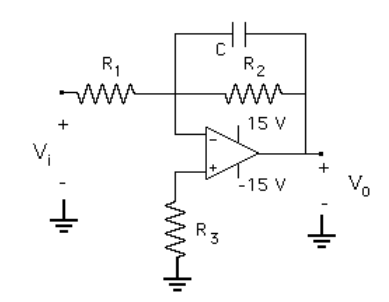
\includegraphics{Img/2_6}\\
		
		\noindent Para la frecuencia de corte se tiene que:\\
		
		\begin{equation}
			\notag f_C = \frac{1}{2\pi R_2 C} = \frac{1}{2 \pi(10nF)(10k\Omega)} = 1591.55Hz
		\end{equation}\\
	
		\noindent En la gráfica se ve claramente que alrededor de $1591.55Hz$ se disminuye a aproximadamente $70\%$ del voltaje y sigue en disminución, esto se debe a que esta configuración sólo permite que se mantenga la diferencia de potencial a bajas frecuencias.\\
		
		\item La frecuencia de corte del filtro pasa bajo alto de la figura 2.7\\
		
		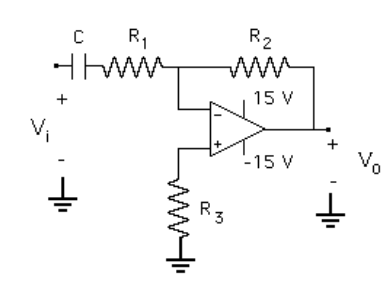
\includegraphics{Img/2_7}\\
		
		\noindent La frecuencia de corte en este caso será:\\
		
		\begin{equation}
			f_C = \frac{1}{2\pi R_1 C} = \frac{1}{2\pi (1k\Omega) (100nF)} = 1591.55Hz
		\end{equation}\\
	
		\noindent Al igual que en la configuración anterior, la frecuencia de corte en la gráfica muestra cuando el voltaje está más del $70\%$, sin embargo, en este caso a partir de este punto se sigue aumentando y se permiten sólo las diferencias de potencial de alta frecuencia, también se evidencia que si se eleva demasiado la frecuencia también se atenúa el voltaje hasta hacerse cero.\\
		
		\item Sistemas trifásicos:\\
		
		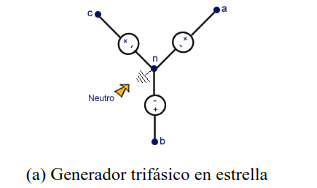
\includegraphics{Img/2_4_a}\\
		
		\begin{itemize}
			\item Carga estrella:\\
			
			\noindent En las gráficas de esta configuración se puede apreciar cómo cada una de las resistencias está en fase con una de las fuentes, eso se debe a que cada una de esas cargas/resistencias está en la misma línea que una fuente.\\
			
			\item Carga delta:\\
			
			\noindent En este caso se puede evidenciar que debido a que ninguna carga está conectada en serie con una fuente, no tendrán el mimo voltaje pico que las fuentes, además, al estar conectadas a dos nodos cada una, se encontrá con que en determinados momentos una resistencia tendrá una diferencia de potencial de aproximadamente el doble del voltaje de una fuente, esto se debe a que las fuentes tienen el mismo voltaje pico el cual afecta a todas las resistencias.\\
			
			
		\end{itemize}
	
		\item Filtro pasa alto a frecuencias altas:\\
		
		\noindent Lo que pasa con él es que a bajas frecuencias el capacitor se carga raápidamente por lo que las bajas frecuencias son eliminadas, sin embargo, pasa algo curioso, ya que a altas frecuencias la oscilación de la onda es tan grande y el cambio de voltaje tan brusco que el capacitador también filtra esas frecuencias.\\
		
	\end{enumerate}
	
	\newpage
	
	\begin{center}
		\textbf{\large CONCLUSIONES}\\
	\end{center}
	
	Inserte conclusiones
	
	\newpage
	
	\begin{center}
		\textbf{\large BIBLIOGRAFÍA}\\
	\end{center}
	
	Guía rápida de PSPICE versión 9.1. Universidad Pontificia de Comillas.\\
	http://dea.unsj.edu.ar/sredes/ManualSpice.pdf
	
	\newpage
	
	\begin{center}
		\textbf{\large ANEXOS}\\
	\end{center}
	
\end{document}